\documentclass[a4paper,twoside,liststotocnumbered]{scrartcl}

% packages importieren
\usepackage[T1]{fontenc}
\usepackage[utf8x]{inputenc}
\usepackage[ngerman]{babel}
\usepackage{todonotes}
\usepackage{float}
\usepackage{graphicx}
\usepackage{pdfpages}
\usepackage[a4paper,bottom=40mm]{geometry}
\usepackage{fancyhdr}
\usepackage{listings}
\usepackage{wrapfig}
\usepackage{tocloft}
\usepackage[acronym,footnote,description,nonumberlist]{glossaries}
\usepackage{enumitem}
\usepackage{textpos}
\usepackage[bookmarks=true,unicode=true,bookmarksopen=true,bookmarksnumbered=true,pdfpagelabels=false,hidelinks=true,bookmarksopenlevel=2]{hyperref}
\usepackage{bookmark}

% sprache auswählen
\selectlanguage{ngerman} 

% empty einstellungen verwenden
\pagestyle{empty}

% default einstellungen von header und footer löschen
\fancyhf{}

\newcommand{\activatefooter}{
	\fancyfoot[RE]{\thepage}
	\fancyfoot[LO]{\thepage}
	\fancyfoot[RO]{Christof Würmli, Sandro Ropelato}
}
\newcommand{\deactivatefooter}{
	\fancyfoot[RE]{}
}

% funktion zum einfügen einer komplett leeren seite
\newcommand{\emptypage}{
	\newpage
	\thispagestyle{empty}
	\mbox{}
}

% selbst definierte farben
\definecolor{light-gray}{rgb}{0.9, 0.9, 0.9}
\definecolor{blue-gray}{rgb}{0.87, 0.89, 0.92}
\definecolor{dark-blue-gray}{rgb}{0.43, 0.44, 0.46}
\definecolor{dark-blue}{rgb}{0.2, 0.2, 0.7}

% für syntax highlighting
\lstset{
	language=C++,
	basicstyle=\footnotesize,
	commentstyle=\color{dark-blue-gray}\it,
	numbers=none,
	backgroundcolor=\color{blue-gray},
	frame=shadowbox,
	xleftmargin=8pt,
	framexleftmargin=5pt,
	xrightmargin=8pt,
	framexrightmargin=8pt,
	framextopmargin=5pt,
	framexbottommargin=5pt,
	tabsize=4,
	captionpos=b,
	breaklines=true,
	breakatwhitespace=true,
	breakautoindent=true,
	title=\lstname,
	inputencoding=utf8x,
	extendedchars=\true,
	showstringspaces=false
}

% übersetzung einiger begriffe
\deftranslation[to=ngerman]{Glossary}{Glossar}

% umlaute
\PrerenderUnicode{Ä}
\PrerenderUnicode{Ö}
\PrerenderUnicode{Ü}
\PrerenderUnicode{ä}
\PrerenderUnicode{ö}
\PrerenderUnicode{ü}

% set document information
\author{Christof Würmli, Sandro Ropelato}
\title{Fahrsimulator}
\hypersetup{pdftitle={Projektarbeit Fahrsimulator},pdfauthor={Christof Würmli, Sandro Ropelato}}

% einrücken beim beginn eines neuen absatzes verhindern
\setlength{\parindent}{0pt}

% glossar erstellen
\makeglossaries
\defglsdisplayfirst[main]{#1#4\protect\footnote{#2}}
\newglossaryentry{opengl}{
	name={OpenGL},
	description={Opensource Grafikbibliothek}
}
\newglossaryentry{directx}{
	name={DirectX},
	description={Microsofts Grafikbibliothek und Konkurrenz zu OpenGL}
}
\newglossaryentry{ogre}{
	name={OGRE},
	description={Object-Oriented Graphics Rendering Engine}
}
\newglossaryentry{mit-lizenz}{
	name={MIT-Lizenz},
	description={Eine vom Massachusetts Institute of Technology entworfene Lizenz zur Benutzung von Software. (Quelle: http://en.wikipedia.org/wiki/MIT\_License, Abruf: 03.12.2011)}
}
\newglossaryentry{shader}{
	name={Shader},
	description={Programm, welches auf der GPU läuft und der Berechnung von Licht-, Schatten- und weiteren Effekten von Materialien dient}
}
\newglossaryentry{szenengraph}{
	name={Szenengraph},
	description={Datenstruktur zur hierarchischen Organisation von von Objekten}
}



% formatierung für index der fussnote
\renewcommand{\thefootnote}{(\arabic{footnote})}

% seitenzahlen mit arabischen ziffern
\renewcommand{\thesection}{\arabic{section}}

% aufbau des dokuments
\begin{document}

	% titelseite
	%
% Titelseite der Projektarbeit
%

\begin{titlepage}
\vspace{4em}
\center

\Large{\textsf{Projektarbeit}}
\vspace{1em}

\Huge{\textsf{Fahrsimulator}}
\vspace{2em}
\\
\Large{
	\textsf{
		Sandro Ropelato (ropelsan)\\
		Christof Würmlil (wurmlchr)\\
		\vspace{2em}
		\today\\
		\vspace{2em}
		Studiengang: Systeminformatik SI\\
		Betreuender Dozent: Peter Früh (frup)
	}
}

\end{titlepage}

	\emptypage
	
	\setcounter{page}{1}
	\section*{Zusammenfassung}
In Zusammenarbeit mit der ETH-Zürich wurde, für eine bestehende Hardwareumgebung, ein Fahrsimulator entwickelt. Die ETH Zürich forscht im Rahmen verschiedener Themen im Gebiet des Strassenverkehrs. Und benötig für diese Zwecke einen Fahrsimulator, in dem möglichst realistische Verkehrssituationen nachgestellt werden können. \\
Die Hardwareumgebung besteht aus einem Cockpit, das mit einem Steuerrad, Gas- , Brems- und Kupplungspedal bestückt ist, einem Projektor und einem Computer. \\
Unter Verwendung einer Open Source Graphik Engine wurde eine virtuelle Welt geschaffen. Durch Eingaben im Cockpit kann das Fahrzeug durch die virtuellen Welt navigiert werden. Ein besonderes Augenmerk wurde auf eine kurze Reaktionszeit zwischen Ein- und Ausgabe sowie ein möglich intuitives Fahrverhalten des Fahrzeuges gelegt. Im Simulator stehen zwei Ansichten zur Verfügung. Eine Ansicht ist diejenige eines Fahrers durch die Windschutzscheibe des Fahrzeugs und die andere ist eine Drittperson Ansicht bei der die Kamera über dem Auto schwebt. Es stehen zudem zwei verschiedene virtuelle Welten zur Verfügung. Die Stadtumgebung beinhaltet mehrere Strassen die sich kreuzen. An Kreuzungen herrscht eine übliche Verkehrsführung, gekennzeichnet durch Asphaltsymbole und Strassentafeln. Die Strasse in der Berglandschaft beschreibt einen Rundkurs, der sich abwechslungsweise in Tunnels im den Berg oder an der Oberfläche befindet.\\
Alle aktuellen Eigenschaften und Eingaben die im Cockpit gemacht werden, werden für eine Auswertung gespeichert. 
\newpage
\section*{Abstract}
In cooperation with ETH Zurich a software for a driving simulator has been developed to go with an existing setup of hardware equipment. ETH is doing research on various subjects and therefore needs a driving simulator which offers the possiblility to simulate certain traffic situations as realistically as possible.\\
The hardware setup consists of a cockpit with a steering wheel, throttle, break and a clutch pedal, a projector and a computer.\\
Using an open source graphics engine a virtual world has been created. Using the input devices in the simulator a vehicle can be controlled within that world. The focus was on minimizing the time delay between the system's input and output and on creating a driving experience as intuitive as possible. The simulator offers two points of view. A first person view which gives the driver the experience of actually sitting inside the vehicle and a third person view with a chase camera positioned outside the car. Furthermore the user can choose between two virtual worlds. A city world containing a road system with traffic signs following the Swiss traffic rules. The second world represents circuit in a mountain region with tunnels.\\
All properties and system inputs are logged in a file for later analysis.

	% eigenständigkeitserklährung
	
\includepdf{src/erklaerungpa.pdf}

	\pagestyle{fancy}
	% header und footer konfigurieren
	\renewcommand{\sectionmark}[1]{\markboth{\thesection{} #1}{}}
	\fancyhead[RE]{\leftmark}
	\fancyhead[LO]{Projektarbeit Fahrsimulator}

	% inhaltsverzeichnis
	\setcounter{page}{1}
	\addtocontents{toc}{\protect\thispagestyle{fancy}}
\tableofcontents

	
	\emptypage

	% hauptteil
	\setcounter{page}{3}
	\fancyhead[RE]{Kapitel \leftmark}
	\activatefooter
	\section{Einleitung}
\subsection{Ausgangslage}

Im Bereich der Fahrsimulatoren gibt es eine Vielzahl von verschiedenen Lösungen. Einige davon bestehen aus Filmmaterial, das abgespielt wird und der Fahrer muss auf die Bremse drücken, sobald ein bestimmtes Ereignis eintritt. Andere Fahrsimulationen bringen bereits eine virtuelle Welt mit, in der man sich mehr oder weniger frei bewegen bzw. frei fahren kann. Jedoch sind bei den meisten dieser Fahrsimulatoren bereits feste Szenarien implementiert, die  nicht geändert werden können. Die Möglichkeiten eines Fahrsimulators werden hauptsächlich durch die Leistungsfähigkeit des Rechners, auf dem die Simulation laufen soll, limitiert. Eine besondere Herausforderung ist die Simulation von Verkehr auf den Strassen. \\
Dieses Projekt wird in Zusammenarbeit mit der ETH Zürich durchgeführt. Im Rahmen unterschiedlicher Forschungsthemen sollen Probanden im Fahrsimulator verschiedene Strassensituationen antreffen. Eine dieser Forschungen bezieht sich auf die Auswirkung von Medikamenten im Strassenverkehr. Hierbei soll die Aufmerksamkeit und Reaktionsfähigkeit des Probanden vor und nach der Einnahme von Medikamenten getestet werden. Eine weitere Forschung untersucht die Augenreaktion beim Einfahren in Tunnels mit einem Fahrzeug. Wenn der Portalbereich eines Tunnels von der Sonne beschienen wird, ist dieser sehr hell, der innenbereich des Tunnels hingegen ist dunkel. Der Autofahrer ist also einem starken Helligkeitunterschied ausgesetzt und die Augen müssen sich auf die neue Situation einstellen. Um herauszufinden, wie sich diese Anpassungsphase der Augen auf die Wahrnemungsfähigkeit und Reaktionfähigkeit auswirkt, werden solche Versuche im Simulator durchgeführt. \\
Die Hardwarekomponenten des Fahrsimulators bestehen aus einem Rechner, einem Beamer, einer speziell bemalten Wand die als Projektionsfläche dient und einem Cockpit mit Autositz und Sicherheitsgurt. Im Cockpit befinden sich Gas- und Bremspedas sowie eine Kupplung, ein Steuerrad mit verschiedenen Knöpfen und eine Gangschaltung. Auf dem Rechner befindet sich eine LabVIEW-Umgebung. Es existiert bereits ein LabVIEW-Programm, das eine Anbindung an das Cockpit macht.

\subsection{Aufgabenstellung}
\subsubsection{Formulierung}
Um die ETH bei ihren Forschungen zu unterstützen wird im Rahmen dieser Projetkarbeit ein Fahrsimulator für die bestehende Hardwareumgebung entwickelt. Durch Manipulationen im Cockpit soll der Proband das Fahrzeug durch eine 3D-Umgebung bewegen können. Die Fahrsimulation sollte dem Probanden die Illusion des Autofahren möglichts realistisch vermitteln. Durch den Einsatz von Google 3D Warehouse wird diese unterstützt. Zudem sollen alle Betriebszustände und Benutzereingaben registriert und aufgezeichnet werden um eine genaue Auswertung zu ermöglichen. 

\subsubsection{Aufteilung der Arbeit}
In einem ersten Schritt wird die Schnittstelle zwischen dem Cockpit und dem zu realisierenden Programm über LabVIEW implementiert. Zur Visualisierung wird ein Video-Player entwickelt, der bei Betätigung des Gas- und Bremspedals die Abspielgeschwindigkeit des Videos angepasst. Beim Video-Player soll zudem die Speicherung von Daten in Log-Files  implementiert werden. Danach wird mit der erstellten Schnittstelle der Fahrsimulator realisiert. Ist dieser implementiert und getestet, werden verschiedene Szenen erstellt. 

\subsection{Grober Zeitplan}
Die ersten zwei Wochen werden dazu vewendet die Simulationsumgebung und dessen Anbindung kennenzulernen. Danach werden weiter vier Wochen eingeplant um die Schnittstelle zwischen dem Cockpit und dem zu realisierendem Programm zu implementieren und sie mit einem Videplayer zu testen. Für den Fahrsimulator und die zu erstellenden Szenen werden ca. vier Wochen eingeplant. Die letzten vier Wochen werden die Dokumentation und eventuelle Ergänzungen benötigt. Der detailierte Zeitplan ist im Anhang F zu finden. 
	\section{Aufbau des Systems}
\subsection{Systembeschreibung}

% Bild für Systembeschreibung
\begin{figure}[H]
\centering 
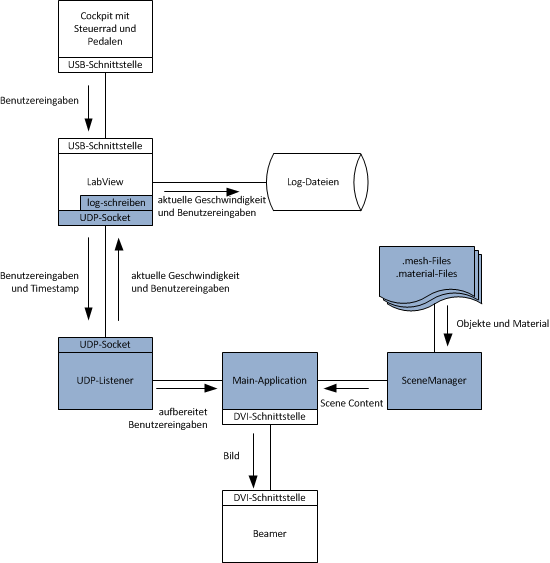
\includegraphics{src/Systembeschreibung.png}
\caption{Systembeschreibung} % Titel der Grafik
\label{Systembeschreibung} % Labelname
\end{figure}


Der Aufbau des Systems für den Fahrsimulator wird anhand der Abbildung \ref{Systembeschreibung} ilustriert. Die blau markierten Komponenten werden im Rahmen dieser Projekt Arbeit entwickelt. Alle übrigen sind bereits vorbestehend. 
Benutzereingaben, die im Cockpit gemacht werden, werden von einem LabView Programm eingelesen. Nun benötigt es einen UDP-Port,  über den verschiedenen Eingaben an das Programm weitergeleitet werden. Es handelt sich hierbei um Werte, die das Drehen des Steuerrades und den Druck auf Gas- oder Bremspedal quantifizieren. Zusätzlich wird der UDP-Port auch für das Empfangen diverser Log-Daten, die von unserem Programm gesendet werden, verwendet. Damit die Empfangenen Daten sauber in ein Log-File geschrieben werden, wird das LabVIEW Programm erweitert. 
Weiter  muss in Programmiersprache C einen UDP-Socket mit entsprechendem UDP-Listener implementieren werden, um die Benutzereingaben zu empfangen. Gleichzeitig wird der UDP-Listener dazu verwendet die Geschwindigkeit des Fahrzeugs sowie Timestamps und weitere Daten an das LabVIEW Programm zurück zu schicken. Damit können die Daten gespeichert und später ausgewertet werden.
\\
Diese Aufteilung durch eine Netzwerkschnittstelle ermöglicht es,  das System, wenn notwendig, zu dezentralisieren. Einfachheitshalber wurde der UDP-Listener erst in einem Video-Beispiel implementier und getestet (Siehe Anhang B). Nachfolgend wird dieser UDP-Listener auch in das Programm des Fahrsimulator transferiert.
Sind die Daten vom UDP-Listener empfangen und aufbereitet, werden sie im Hauptprogramm (Main Application) weiter verwendet. Während die Position des Steuerrades, des Gas und Bremspedales vom UDP-Listener permanent an das Hauptprogramm übertragen werden, wertet dieses die Positionen aus und veranlass die entspechenden Aktionen in der geladenen Szene. 
Die Szene selbst wird von einem Szenen-Manager geladen. Dieser benötig für die zu ladenden Objekte ein Meshfiles und mindestens ein Materialfile. Die Form jedes Objektes in der Szene wird durch ein separates Meshfile definiert. Texturen und Materialien werden durch ein oder mehrere Materialfiles beschrieben. Ein Materialfile kann zur Beschreibung unterschiedlicher Objekte verwendet werden. Die berechnete Szene wird schlussendlich in einem Fenster von Hauptprogramm angezeigt und über eine DVI-Schnittstelle an den Beamer übertragen. Der Beamer projeziert das Bild an die Wand, die sich direkt vor dem Cockpit befindet. 

\subsection{Anforderungen}
\subsubsection{Funktionale Anforderungen}
\begin{itemize}
\item Der Proband kann das Fahrzeug im Fahrsimulator durch manipulation am Steuerrad und der Pedalen im Cockpit steuern.
\item Die aktuelle Geschwindigkeit der Fahzeuges wird dem Probanden angezeigt.
\item Es sollen zwei unterschiedliche Szenen zur verfügung gestellt werden.  Die eine Szene sollte eine Stadt darstellen und die andere Szene eine Landschaft mit Tunnels.
\item Die manipulationen des Benutzers und wichtige Parameter wie z.B. Geschwindigkeit sollen in einer Datei aufgezeichnet werden um diese auszuwerten.
\item Alle ein- und ausgehenden Parameter des System sollen in LabVIEW verfügbar sein um diese auswerten und kontrollieren zu können. 
\end{itemize}

\subsubsection {Nicht Funktionale Anforderungen}
\renewcommand{\labelenumi}{\alph{enumi})}

\begin{itemize}
\item Das System soll robust sein. 
\item Das Starten des Fahrsimulator sollte möglichst einfach gehalten werden. Das Steuer des Fahrzeuges soll möglichst intuitiev sein wie man es sich von einem richtigen Fahrzeug gewöhnt ist. 
\item Der Fahrsimulator soll dem Probanden eine möglichst realistische Fahrsimulation bieten in der sich Strassen und verschiedene Objekte befinden.
\item Die Raktionszeit des Systems soll möglichst klein sein. Die Verzögerung des Systems soll mess-  und kalkulierbar sein.
\item Das System soll möglichst Modular aufgebaut sein um später einfach erweitert werden zu können.
\item Das System soll auf der existierender Hardware funktionieren, soll aber auch noch lauffähig sein wenn Teile des Fahrsimulators ausgetauscht werden. 
\end{itemize}

	\section{Realisierung}
Wie bereits in der Systembeschreibung beschrieben, wird der Fahrsimulator in drei Hauptkomponenten unterteilt, den UDP-Listener, den Szenen-Manager und das Hauptprogramm. Da die Verbindung zwischen dem Cockpit und dem Fahrsimulator mit einer Netzwerkschnittstelle realisiert wird, ist es möglich die Anbindung an das Cockpit und den Fahrsimulator physisch auf zwei unterschiedlichen Rechnern zu betreiben. Eine Alternative ist die Umsetzung mit dem \gls{ogre}-Framwork (Siehe Anhang C). Dieses Framework bietet umfassende Lösungen um Steuerradär und Pedalen, wie sie in userem Cockpit vorhanden sind, anzusteuern.\\
Da die 3D-Umgebung mit fortscheitendem Projekt ausgebaut wird, könnte sich die notwendige Rechenleistung erheblich steigern. Folgen ungenügender Leistung sind unregelmässige Bewegungen (Lags) in der virtuellen Umgebung oder sogar bis zum Absturz des gesamten Programms führen.\\
Aus diesem Grund ist die erste Variante mit der Netzwerkschnittstelle für das Fahrsimulatorprojekt besser geeignet. Die andere Variante wird verworfen.
\subsection{LabVIEW Programm}
Eine LabVIEW-Umgebung existiert bereits auf dem Rechner, an den das Cockpit angeschlossen ist. Dazu existierte ein LabVIEW-Programm, welches bereits die Eingaben im Cockpit einliest. Da dieses Programm jedoch nicht genau den Anforderungen entspricht, wird ein neues LabVIEW-Programm realisiert. Dieses Programm wird so erweitert, dass diese Eingaben in Form von definierten Parametern als UDP-Packet in regelmässigen Zeitabständen gesendet werden. Zusätzlich wird ein zweiter UDP-Socket eingerichtet um Packete, die vom Fahrsimulator gesendet werden, zu empfangen. Die Daten der empfangenen Packete werden von LabVIEW in ein Log-File gespeichert.
% ev Bild
\subsection{UDP-Listener}
\label{sec:udp-listener}
Die Paramter werden vom LabVIEW-Programm permanent gelesen und ca alle 0.01 Sekunden wird ein UDP-Packet gesendet. Um die Zeit zwischen der Eingabe des Probanden und derReaktion des Fahrzeuges im Simulator möglichst gering zu halten, müssen ankommende Packete sofort gelesen werden. Angesitchts der hohen Anzahl an Datenpacketen pro Zeitraum, ist es vernachlässigbar, wenn einige Packete verloren gehen oder vertauscht werden. Das UDP-Protokoll gewährleistet genau diese Eigenschaften.

\begin{figure}[H]
\centering 
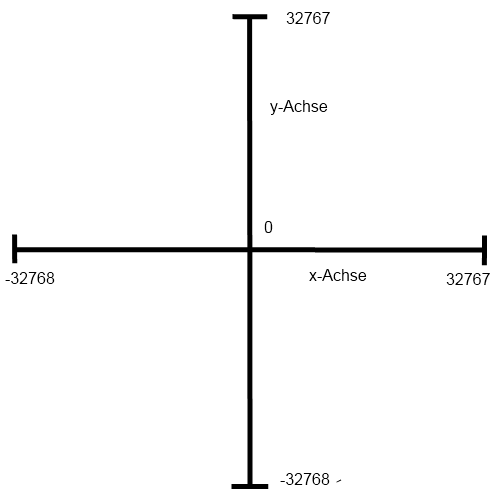
\includegraphics[scale=0.5]{src/koordinatensystem.png}
\caption{Koordinatensystem} % Titel der Grafik
\label{Koordinatensystem} % Labelname
\end{figure}

Die von LabVIEW empfangenen Daten sind in erster Linie Parameter die den Zustand der Pedalen und des Steuerrades representieren. Die beiden Pedalen werden in einem Koordinatensystem wie in Abbildung \ref{Koordinatensystem} auf der y-Achse abgebildet. Die positive y-Richtung quantifiziert das Gas und die negative y-Richtung das Bremspedal. Die Intensität beider Pedalen wird durch 32767 bzw. 32768 ganzzahlige Werte identifiziert. Wenn also keines der beiden Pedalen gedrückt ist, wird dies durch den y-Wert 0 dargestellt. Ein voll gedrücktes Gaspedal entspricht dem y-Wert 32767 und dementsprechend ein voll gedrücktes Bremspedal dem Wert -32768. Der x-Wert im Koordinatensystem quantifiziert den Einschlagswinkel des Steuerrades. Ist das Steuerrad in der neutralen Stellung, entspricht dies dem x-Wert 0. Wenn das Steuerrad vollständig nach rechts eingeschlagen ist, wird dies durch den positiven x-Wert 32767 identifiziert. Umgekehrt wird ein vollständiger Einschlag nach links durch den negativen x-Wert -32768 identifiziert. Es können zusätzlich weitere Parameter wie Tastendrücke am Steuerrad, übermittelt werden, wenn dies erforderlich sein sollte. Zusätzlich zu den Parametern des Cockpits wird von LabVIEW auch noch ein Timestamp gesendet. Der Timestamp wird von UDP-Listener empfangen und nach dem Abspeichern der Parameter wieder zurückgeschickt. Somit kann festgestellt werden, wieviel Verzögerung die Netzwerkschnittstelle verursacht. \\
Da das LabVIEW-Programm und der Simulator nicht synchronisiert sind, wird der DP-Listener zur Überbrückung verwendet. Der UDP-Listener speichert alle Parameter in Variabeln ab. Diese Variabeln werden vom Hauptprogramm ausgelesen und interpretiert. Dieses auslesen der Variabeln erfolgt nun synchron, da das Hauptprogramm nur dann Daten vom UDP-Listener liest, wenn dieses dazu bereit ist.

\subsection{Virtual Reality}
Eine erste Idee um eine virtuelle Realität zu erzeugen, war ein Einsatz von google Street View oder google Maps. Google Maps bietet die möglichkeit, da die Satelitenbilder von der ganzen Erde gemacht wurden, überall auf der Welt zu fahren. Jedoch ist die Auflösung der Bilder nicht immer genug hoch um diese aus der Sicht eines Fahrers anzeigen zu können. Erschwerend kommt hinzu, dass die Aufnahmen nur von oben gemacht wurden und somit keine Seitenansicht einer steilen Felswand oder eines Hauses zur verfügung steht. Auch werden, da die Fotos aus der Vogelperspektive gemacht wurden, verschiedene Elemente die sich über der Strasse befinden wie zum Beispiel Bäume, Brücken oder Autos auf der Strasse flachgedrückt angezeigt.  Dies bedeutet das kein klare Strasse sichtbar ist. Somit wäre der Einsatz von google maps keine zufriedenstellende Lösung. \\
Eine bessere Auflösung und darstellung der Strassen bietet Google Street View. Hierbei wurd mit einem Wagen, der eine 360 Grad Kamera auf dem Dach montiert hatte, den Strassen entlang gefahren und ca. alle 20 Meter ein Foto gemacht. An einem solchen Punkt an dem ein Foto gemacht wurde, kann der Benutzer nun in alle Richtungen Blicken. Es werden sogar grosse Gegenstände wie Wände oder Hausmauern erkannt und beim drehen der Ansicht interpoliert. Diese interpolierung ist jedoch nicht immer korrekt und führt teilweise zu merkwürdigen Anzeigen. Zudem gibt es zwischen zwei Bildern einen zu grossen Unterschied um eine fliesende Bewegung zu Simulieren. Dies könnte durch eine Interpolation der zwei Bilder gelöst werden was viel Rechenleistung kostet und denoch ein unbefriedigendes Resultat liefert. Denn durch die Interpolation wird die Lücke zwischen den beiden Bildern zwar aufgefüllt, jedoch ist der Übergang derart verschwommen das keine Objekte erkannt werden können. 
%ev. Screenshot
Zudem wurden meist nur auf einer Spur Fotos gemacht. Eine Ausnahme bilden die Autobahnen. Auf allen übrigen Strassen hat man sich darauf beschränkt Fotos nur in eine Richtung zu machen. Wenn man nun in die andere Richtung fahren möchte, sieht es so aus als würde man auf der falschen Seite fahren. Somit kommen einem die anderen Verkehrsteilnehmer, die sich ebenfalls auf den Fotos befinden, entgegen. Auch dieser Lösungsansatz muss deshalb Verworfen werden. Eine weiter möglichkeit besteht darin, dass eine eingene Umgebung entworfen wird.\\
Für den Fahrsimulator wird also eine virtuelle dreidimensionale Umgebung benötigt, in der man sich bewegen kann. Diese Umgebung, auch Szene genannt, setzt sich aus verschiedenen Objekten zusammen. Die Struktur eines solchen Objektes wird duch ein Mesh-File beschrieben. In einer Szene kann das gleiche Objekt mehrmals an verschiedenen Positionen vorkommen. Das Objekt kann durch eine skalierung auch einmal gross und einmal klein erscheinen. Oder man kann sie durch eine Rotation unterschiedlich machen. Zusätzlich wird mindestens ein Material-File benötigt in dem sämtliche Texturen und Materialien, die von Objekten der Szene verwendet werden, definiert sind.
Ein Beispiel von einem Matrial wie es ein einem material-File definiert ist wird im Listing \ref{example_materialfile_material} illustriert.
\begin{lstlisting}[caption={Beispiel aus dem material-File für ein Material},label={example_materialfile_material}]
material city_ground
{
	technique
	{
		pass
		{
			diffuse 0.0 0.0 0.0 1.00
			ambient 0.75 0.75 0.75 1.00	
		}
	}
}
\end{lstlisting}
Nach dem Keyword \textit{material} wird der Name des Materials angegeben. Als \textit{technique}-Block wird hier einer angegeben. Es können mehrere Blöcke angegeben. Diese Blöcke können optional auch Namen gegeben werden um zu identifizieren wofür die einzelnen Blöcke sind. Ausgeführt wird jedoch immer nur einer der Blöcke wobei der erste Block der bevorzugteste ist und der unterste Block die letzte Fallbacklösung wäre. Im \textit{pass}-Block werden die Reflektionswerte und die Farbe angegeben. Es können mehrer \textit{pass}-Blöcke angegeben werden die jeweils hintereinander ausgeführt werden und sich überlagern. Das \textit{ambiant} als ambientes Licht bestimmt grundsätzlich die Farbe des Matierials. Die Zahlen repräsentieren die RGB-Werte und können zwischen 0 und 1 liegen. Die Farbe des Materials in diesem Beispiel ist ein helles Grau. Die vierte Zahl representiert den Alphawert der Farbe. Der Alphawert quantifiziert die Sichtbarkeit des Materials wobei 1.0 voll sichtbar und 0.0 unsichtbar ist. \\

Weiter zeigt das Listing \ref{example_materialfile_texture} die definition einer Textur in einem material-File.
\begin{lstlisting}[caption={Beispiel aus dem material-File für eine Textur},label={example_materialfile_texture}]
material city_street_h
{
	technique
	{
		pass
		{
			diffuse 0.80 0.80 0.80 1.00

			texture_unit
			{
				texture street_h.png 2d 4
				filtering anisotropic
			}
		}
	}
}
\end{lstlisting}
Für die Textur wird in diesem Beispiel kein Ambientes Licht definiert und es wird der Standartwert 0 genommen. Der diffuse Anteil bestimmt wie stark das Material das Licht reflektiert. Da die Textur des Materials gut sichtbar sein soll, fällt dieser Wert relativ hoch aus. Im Block \textit{texture\_unit} wird die Textur angegeben und konfiguriert. Die Graphik die als Textur verwendet wird, wird nach dem Keyword \textit{texture} angegeben. Das erster Argument nach der Graphikdatei, das \textit{2d} konfiguriert die zweidimensionale Graphik als normale zweidimensionale Textur. Die vier als drittes Argument gibt die Anzahl zu generierenden Mipmaps an. Zusätzlich kann ein Filter für die Textur mit dem Keyword \textit{filtering} angegeben werden. Der anisotropische Filter wertet die Qualität der Textur in der Distanz auf. Hierbei wird die Richtung, der die Textur betrachtet wird, berücksichtigt.\\
Es werden zwei unterschiedliche Szenen für den Fahrsimulator erstellt. Die eine Szene zeigt eine Stadt mit Häusern, Kreuzungen und Verkehrsschildern. Die andere Szene stellt eine Berglandschaft mit mehreren Tunnels dar. Die Szenen werden mit dem Programm Cinema4D erstellt. 
\subsubsection{Erstellen der Stadtszene}
\begin{figure}[H]
\centering 
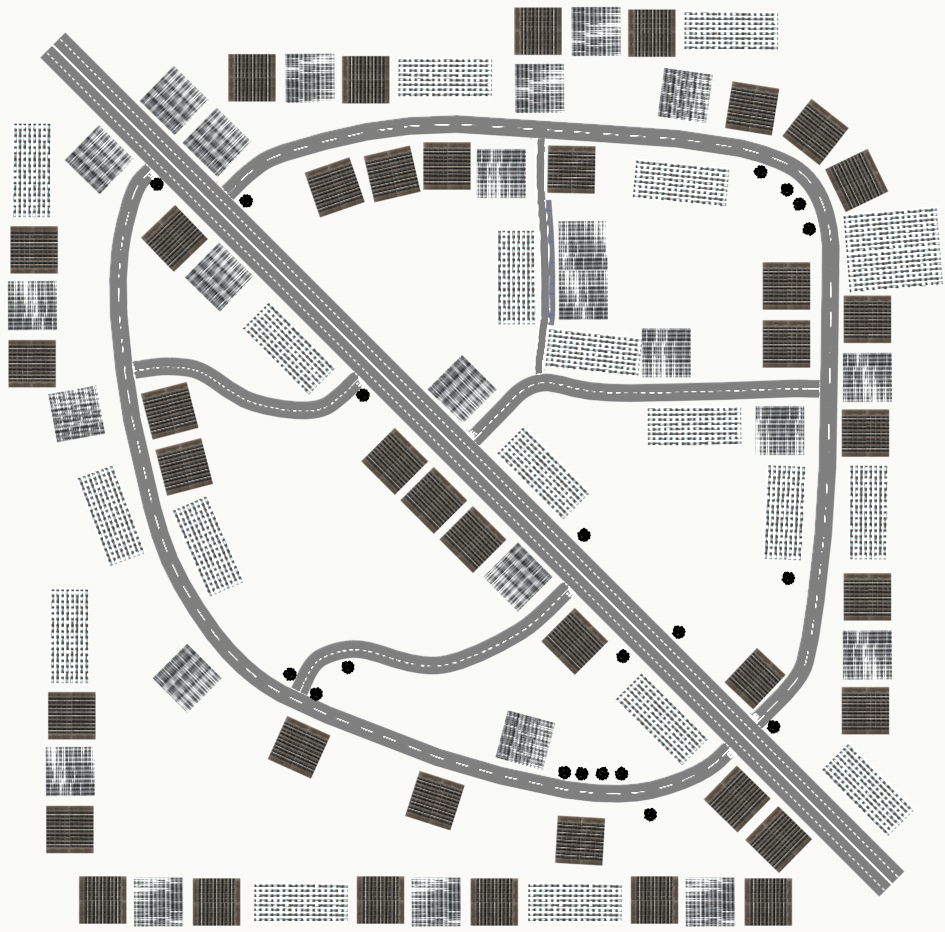
\includegraphics[width=1\linewidth]{src/CityWorld_map.png}
\caption{Karte der Stadtszene} % Titel der Grafik
\label{CityWorld_map} % Labelname
\end{figure}
Um die erstellte Stadtszene gut dokumentieren zu können, zeigt Abbildung \ref{CityWorld_map} eine Übersichtskarte. Die grosse vierspurige Strasse die sich von oben links nach unten rechts durch die gesamte Szene zieht ist eine rechteckige Ebene. Die ebene ist mit einer Textur versehen, die die vier Spuren mit einer Sicherheitelinie in der Mitte darstellt. Die Textur ist jedoch nicht so lange wie die gesammte Strasse. Sie hat nur die Länge von einmal einem Stück mit dem Strich der gestrichelten Sicherheitslinie, die die beiden Spuren die in die gleiche Richtung fahren trennt, und einmal ein Stück ohne dem Strich. Die Textur wird auf der Ebene immer wieder wiederhohlt. Auch bei allen anderen Strassen ist die Textur nur ein kurz und wird wiederholt. Ein Beispiel für eine solche Strassentextur ist in der Abbildung \ref{examples_street_textures} zu finden. \\
\begin{figure}[H]
\centering 
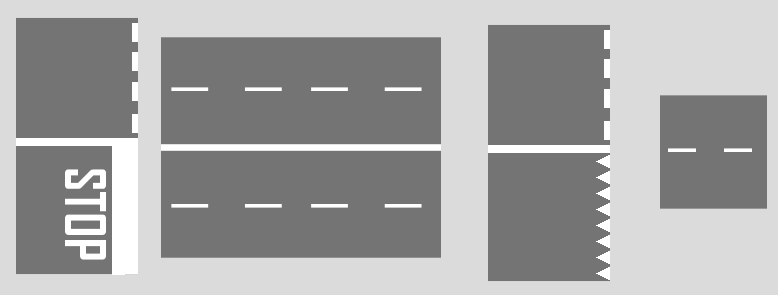
\includegraphics[scale=0.6]{src/examples_street_textures.png}
\caption{Beispiele von Strassentexturen} % Titel der Grafik
\label{examples_street_textures} % Labelname
\end{figure}
Die Strassen mit Kurven werden mit \glspl{spline} beschrieben. Eine Linie wird der \gls{spline} entlangeführt um die Breite einer Strasse zu erhalten. Die Textur der Strasse wird auf dieses, so zusammengefügte, Objekt gelegt. Der Abschluss solcher geschwungenen Strassen bilden wiederum rechteckige Ebenen. Diese erhalten die Textur einer Stoplinie mit Beschriftung auf der Strasse oder den vielen Dreieckigen Zeichen für kein Vortritt wie in Abbildung \ref{examples_street_textures} gezeigt. \\
Zusätzlich zu den Symbolen auf der Strasse, werden noch Verkehrsschilderobjekte in die Szene geladen. Die Abbildung \ref{screenshot_trafficsignal} zeigt ein Beipiel eines solchen Objektes. \\
\begin{figure}[H]
\centering 
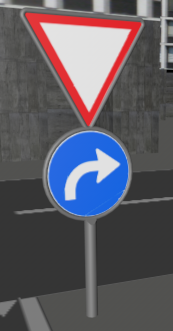
\includegraphics[scale=0.6]{src/screenshot_trafficsignal.png}
\caption{Beispiele eines Verkehrssignals} % Titel der Grafik
\label{screenshot_trafficsignal} % Labelname
\end{figure}

Die Häuser der Stadt sind einfache Blöcke die mit einer Textur von vielen Fenstern versehen werden. Insgesammt sind drei Gebäudetypen, wie in Abbildung \ref{screenshot_buildings} dargestellt,  vorhanden. Diese drei Typen werden einzeln dubliziert eventuell gedreht und in der Szene verteilt. Zusätzlich wird das ETH Zürich Gebäude in der Szene geladen. Dieses Gebäudemodel wurde aus dem Google 3D Warehouse heruntergeladen. Das Objekt wurde in google SketchUp bearbeitet und als eigenes Objekt abgespeichert. Die Bearbeitung heinhaltet vor allem die neuberechnung der Oberflächennormalen und das entfernen der Bodenplatte auf der die ETH Zürich gestanden hat. Die Texturen mussten manuell übernommen werden. Das ETH Objekt wird in die Szene geladen, skaliert und an der richtigen Stelle platziert. 
\begin{figure}[H]
\centering 
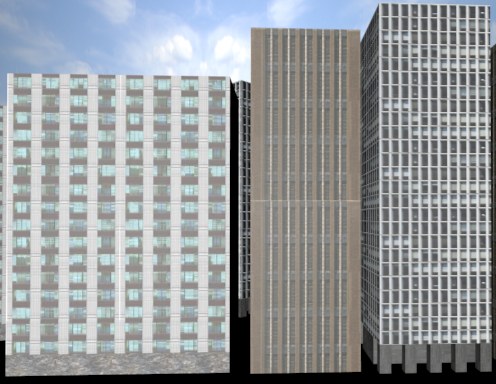
\includegraphics[scale=0.4]{src/screenshot_buildings.png}
\caption{Drei verschidene Gebäudetypen} % Titel der Grafik
\label{screenshot_buildings} % Labelname
\end{figure}
Um der Szene ein bisschen Farbe zu verleihen sind noch Bäume, wie in Abbildung \ref{screenshot_tree} in der Szene vorhanden. Ein Baum besteht aus einem Stamm mit einer Holztextur und einer Krone. Die Krone ist eine zufällig generierte Landschaft die zu einer Kugel geformt wird. Dadurch entstehen die verschiedenartigen Aus- und Einbuchtungen in der Baumkrone. Um die Illusion vollständig zu machen wird darauf eine Textur mit Blättern gelegt.\\

\begin{figure}[H]
\centering 
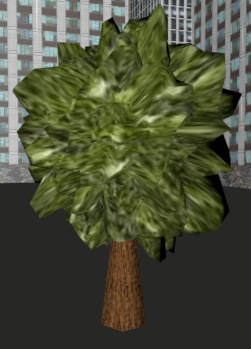
\includegraphics[scale=0.4]{src/screenshot_tree.png}
\caption{Baum} % Titel der Grafik
\label{screenshot_tree} % Labelname
\end{figure}

\subsubsection{Erstellung der Berglandschaft mit Tunnels}
Um die Berglandschaft zu generieren gibt es im Cinema4D ein eigens dafür vorgesehenes Objekt. Durch die Konfiguration des Landschaftsobjekt kann die Höhe und Anzahl der Erhöhungen und Vertiefungen festgelegt werden. Die Strasse in der Berglandschaft wird änlich gemacht wie in der Stadtszene. Zusätzlich wird aber der \gls{spline} ein halber Zilinder mitgegeben der ihr entlangfährt. Der halbe Zilinder wird mit einer Operation versehen damit er, an den Orten an denen die Strasse in der in der Landschaft befindet, diese ausschneidet und ein Tunnel generiert. Die Wand des Tunnels wird mit einer Betonplattenstruktur, wie sie in Abbildung \ref{texture_concretetiles} zeigt, versehen. Die Berglandschaft selbst wird mit einer \gls{seamless} Felsentexture versehen. 
\begin{figure}[htbp]
\centering 
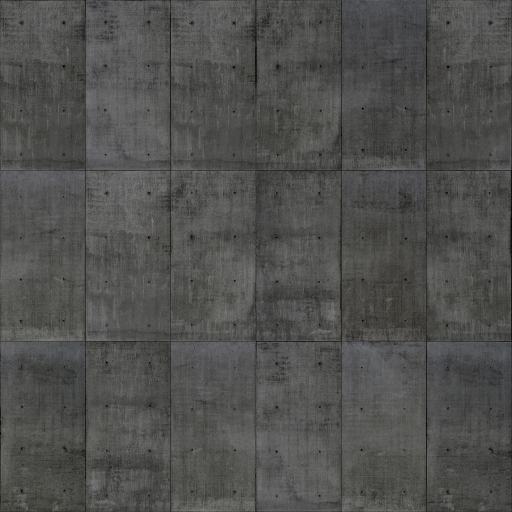
\includegraphics[width=0.4\linewidth]{src/texture_concretetiles.png}
\caption{Tunnelwandtextur} % Titel der Grafik
\label{texture_concretetiles} % Labelname
\end{figure}

\newpage
\subsubsection{Fahrzeug}
Zur Darstellung eines Autos wurde aus dem Google 3D Warehouse ein Mini Cooper heruntergeladen und in nach \gls{ogre-xml}konvertiert. Wie in Abbildung \ref{screenshot_minicooper} zu sehen, wird dieser aus der Perspektive einer dritten Person betrachtet. Beim Rückwärtsfahren wird die Kamera um das Fahrzeug gedreht, so dass man nach hinten sehen kann. Mit der Taste V auf der Tastatur kann die Ansicht in das innere des Fahrzeugs gewechselt werden. Zu Beginn wirde die Kamera lediglich in das innere des Mini Coopers versetzt, dorthin wo der Kopf des Fahrers in etwa sein sollte. In einem zweiten Schritt wurde jedoch ein eigenes Fahrerkabine designed. Dies war vorallem deshalb notwendig, um eine Geschwindigkeitsanzeige implementieren zu können. 
\begin{figure}[H]
\centering 
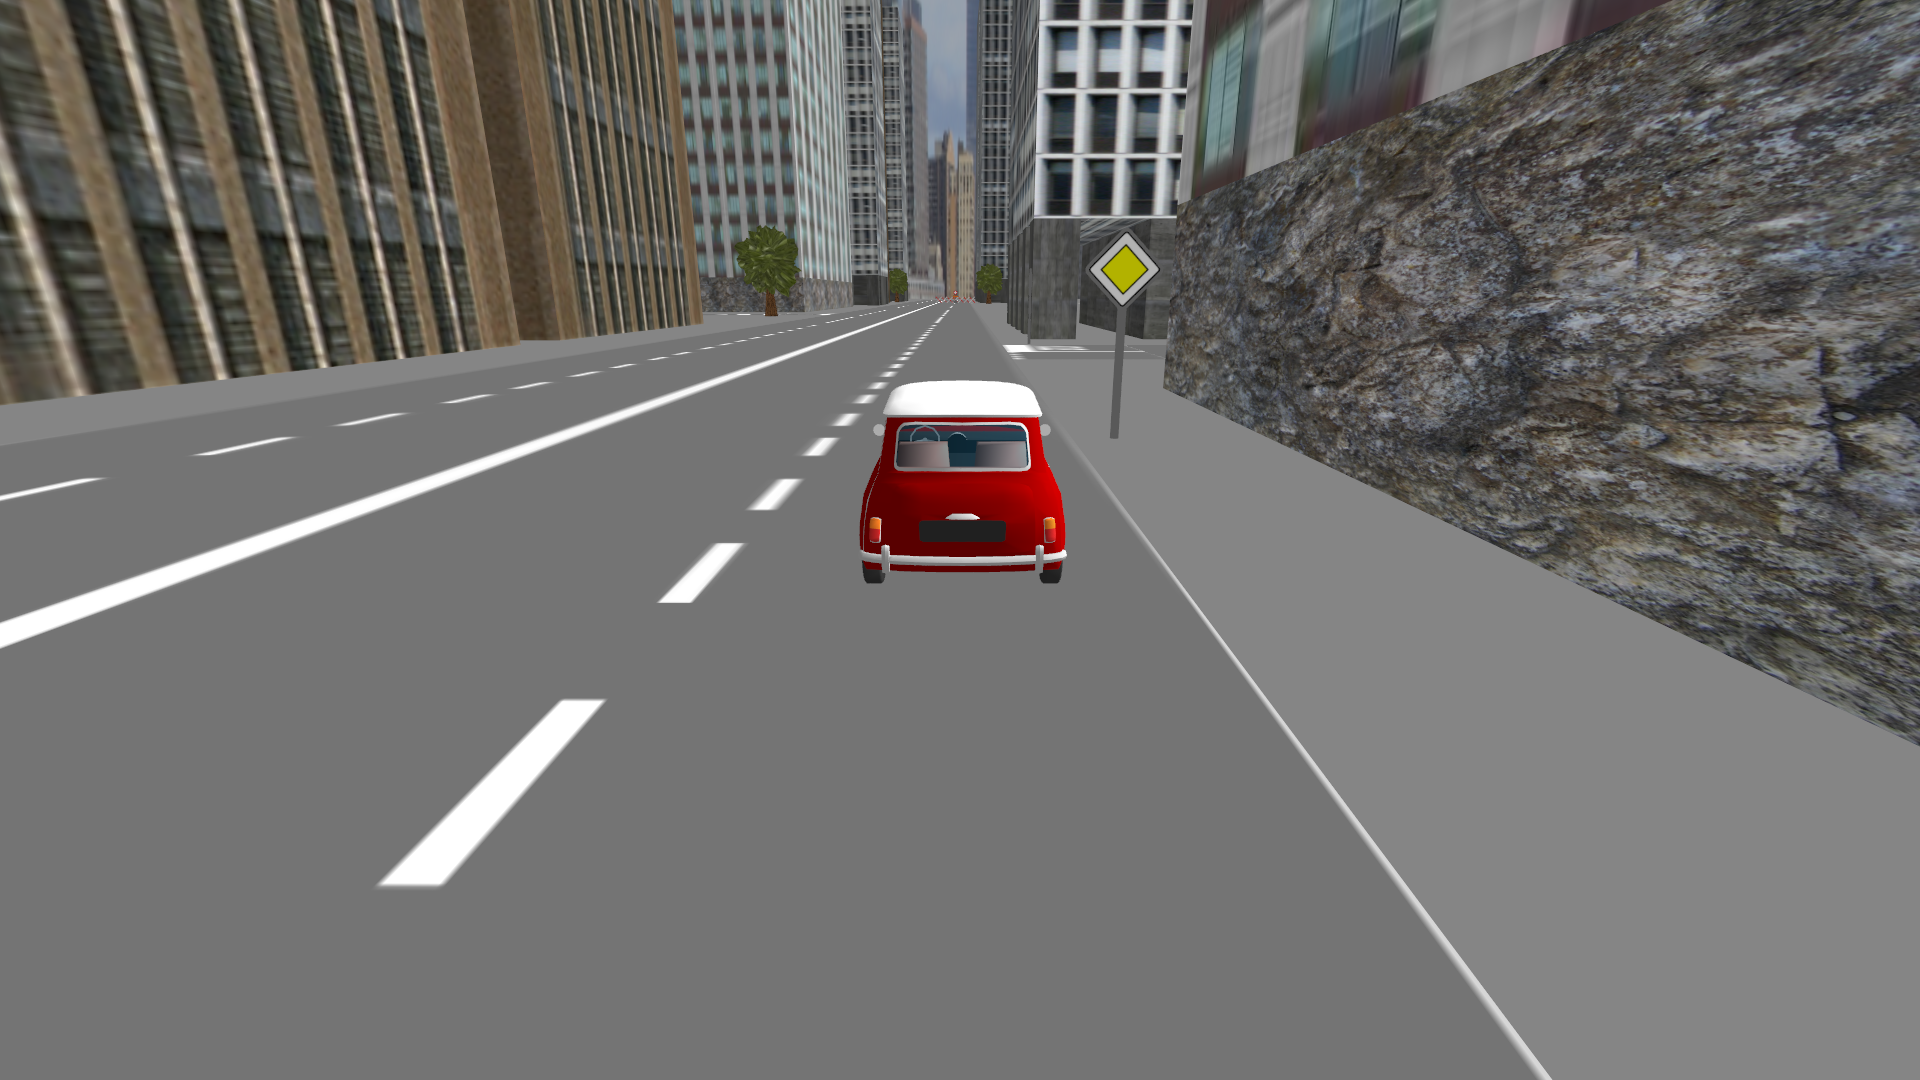
\includegraphics[width=1\linewidth]{src/screenshot_minicooper.png}
\caption{Der Mini Cooper aus der 3rd-Person-Ansicht} % Titel der Grafik
\label{screenshot_minicooper} % Labelname
\end{figure}

\newpage
Wie die Abbildung \ref{screenshot_cockpit} veranschaulicht, ist die Geschwindigkeitsanzeige die mittlere der drei Anzeigen. Sie besteht aus zwei Objekten. Eines der Objekte ist die gesamte Innenansicht selbst und das zweite Objekt ist der rote Zeiger der Geschwindigkeitsanzeige. Dieser wird an der richtigen Stelle Plaziert und wird je nach Geschwindigkeit gedreht. Somit sind zwei Ansichten möglich. Die Sicht des Fahrers mit der eigens dafür erstellten Fahrerkabine und die Aussenansicht in der der Mini Cooper angezeigt wird.
\begin{figure}[H]
\centering 
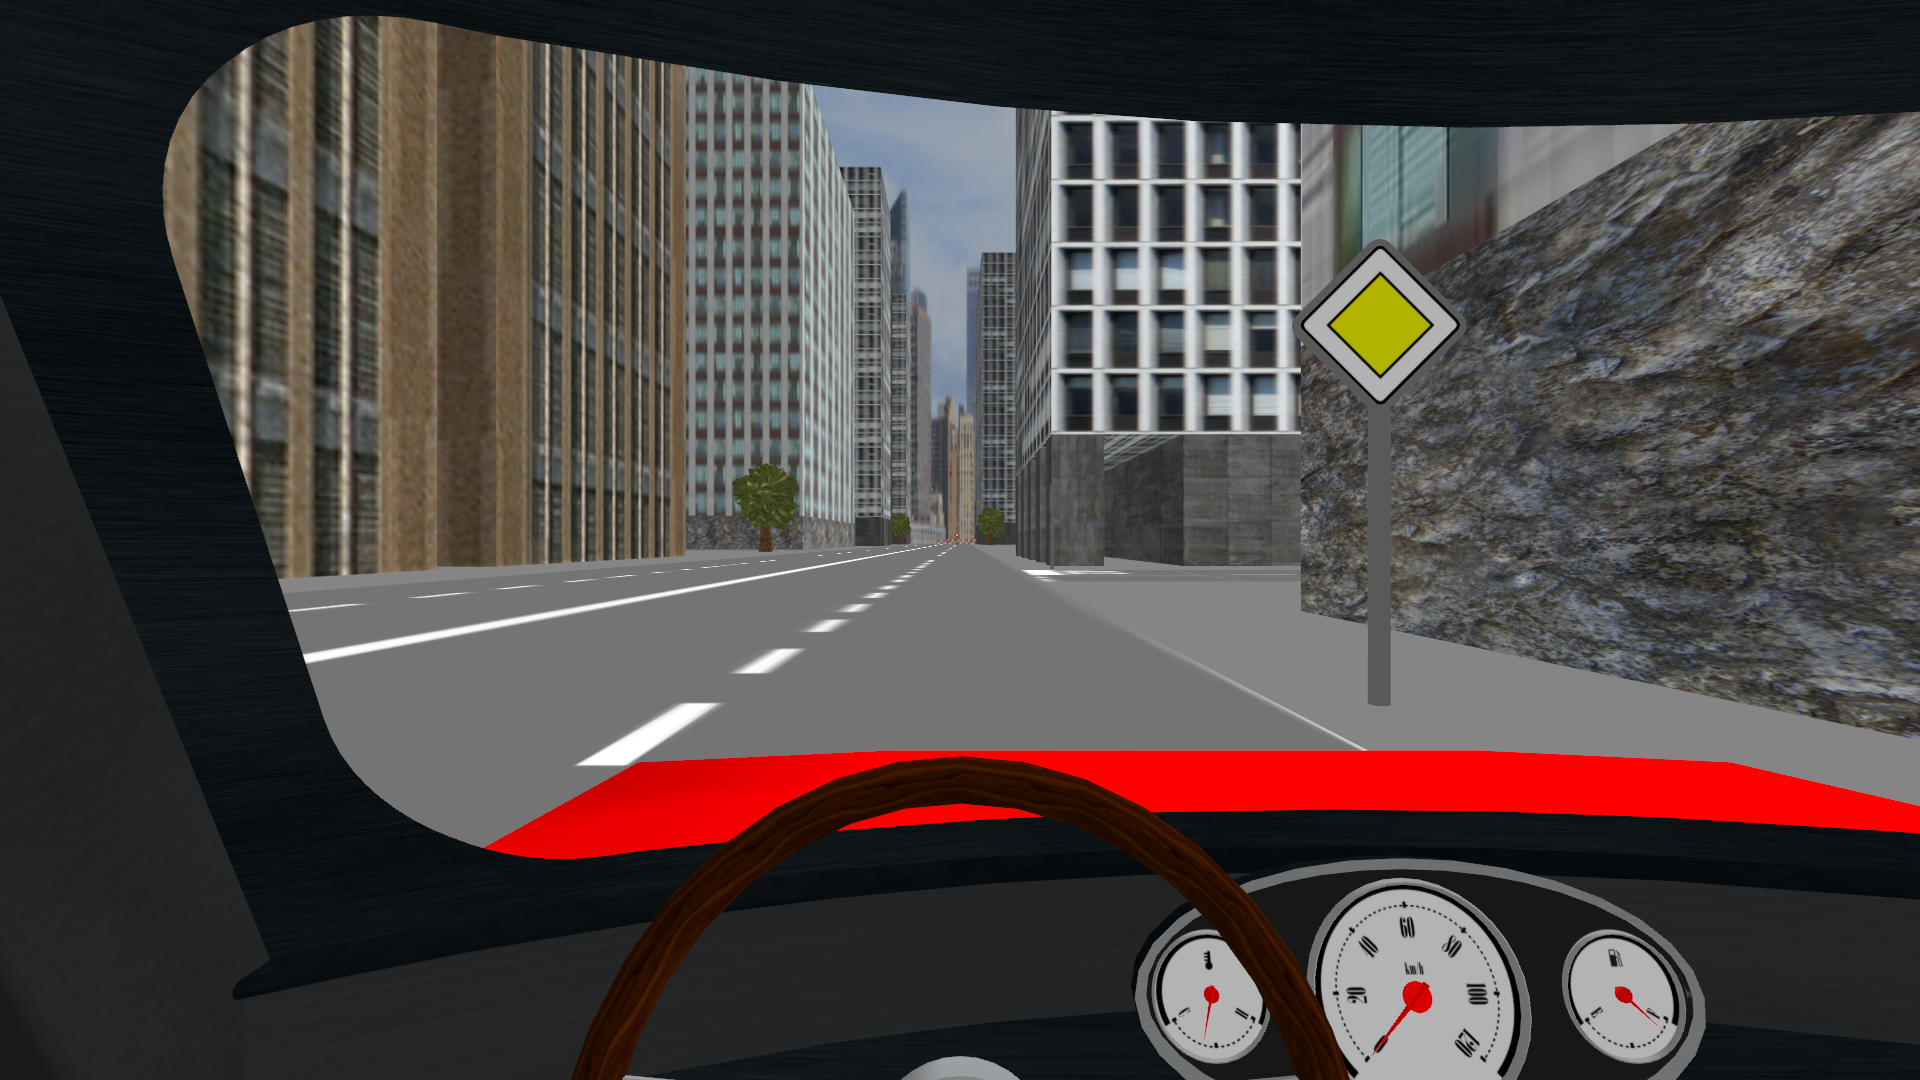
\includegraphics[width=1\linewidth]{src/screenshot_cockpit.png}
\caption{Innenansicht des Mini} % Titel der Grafik
\label{screenshot_cockpit} % Labelname
\end{figure}
Um die Geschwindigkeit des Fahrzeuges herauszufinden, wurde im Cinema4D, in dem alle Szenen erstellt wurden, mit reellen Werten gearbeitet. So wurden Strassen wirklich sechs Meter breit modeliert. Somit konnte auch die Länge der Strasse festgelegt werden. Um die Geschwindigkeit zu ermitteln, wurde in Cinema4D eine Distanz abgemessen und diese mit verschiedenen Konstanten Geschwindigkeiten abgefahren und die Zeit gemessen. Die interne Geschwindigkeit im Programm wird mit einem Faktor in die tatsächliche Geschwindigkeit umgerechnet. Diese kann dann auf dem Tachometer angezeigt werden.\\



\newpage
\subsection{Hautpprogramm}

%Sequenzdiagramm
%Blockdiagramm

\begin{figure}[H]
\centering 
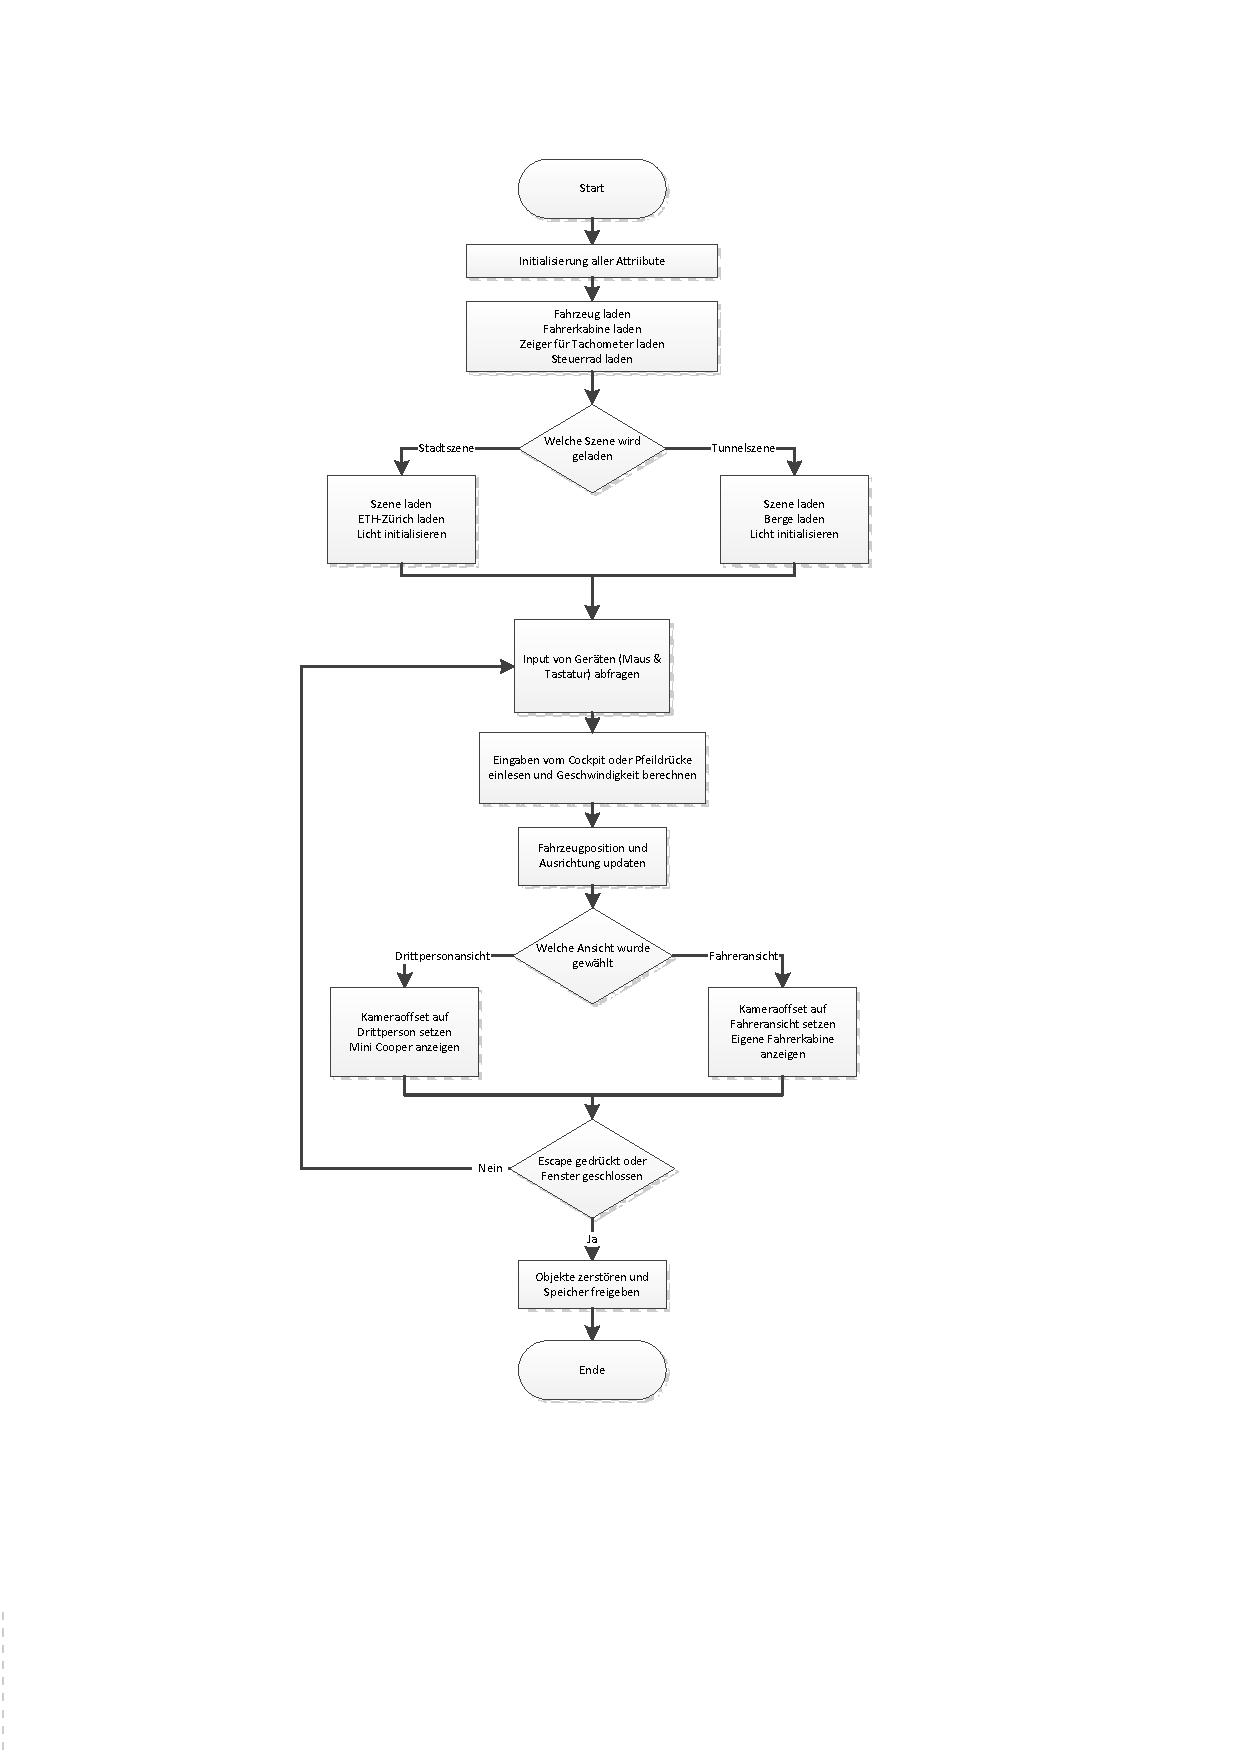
\includegraphics[width=0.6\linewidth]{src/flowchart_mainapplication.pdf}
\caption{Ablauf des Hauptprogramms} % Titel der Grafik
\label{ablauf_hauptprogramm} % Labelname
\end{figure}

\newpage

\subsubsection{Initialisierung}

Beim Start der Applikation werden die Konfigurationsfiles (siehe Kapitel \ref{sec:konfigurationsfiles}) geladen. Aus den darin enthaltenen Informationen wird das Grundgerüst von OGRE erstellt. Dazu gehören folgende Objekte:

\minisec{rootNode}
Der RootNode der 3D-Szene. Alle Objekte sind diesem angehängt.
\minisec{renderWindow}
Das RenderWindow ist das sichtbare Fenster der Applikation. In ihm wird der gesamte grafische Inhalt dargestellt.
\minisec{camera}
Wie der Name vermuten lässt, ist dies die Kamera, durch welche der Benutzer die Szene beobachtet.
\minisec{viewPort}
Der ViewPort ist mit dem Kameraobjekt verknüpft und zeigt die Bildprojektion der 3D-Szene an. 

\begin{lstlisting}[caption={Laden der Konfigurationsdateien},label={laden_konfigurationsdateien}]
// create root node
#ifdef _DEBUG
rootNode = new Ogre::Root("Resources/plugins_d.cfg", "Resources/graphics_d.cfg", "log_d.txt");
#else
rootNode = new Ogre::Root("Resources/plugins.cfg", "Resources/graphics.cfg", "log.txt");
#endif

// load config file
Ogre::ConfigFile configFile;
#ifdef _DEBUG
configFile.load("Resources/resources_d.cfg");
#else
configFile.load("Resources/resources.cfg");
#endif

// load resource files
Ogre::ConfigFile::SectionIterator it = configFile.getSectionIterator();
while(it.hasMoreElements())
{
	Ogre::String sectionName = it.peekNextKey();
	Ogre::ConfigFile::SettingsMultiMap* settings = it.getNext();
	Ogre::ConfigFile::SettingsMultiMap::iterator i;
	for(i = settings->begin(); i != settings->end(); ++i)
	{
		Ogre::ResourceGroupManager::getSingleton(). addResourceLocation(i->second, i->first, sectionName);
	}
}

// try to initialize window with settings from config file
if(!(rootNode->restoreConfig()))
{
	throw Ogre::Exception(Ogre::Exception::ERR_INVALID_STATE, "Could not read graphics configuration", "MainApplication::go");
}

renderWindow = rootNode->initialise(true, "Driving Simulator V1");

// initialize resources
Ogre::TextureManager::getSingleton().setDefaultNumMipmaps(5);
Ogre::ResourceGroupManager::getSingleton(). initialiseAllResourceGroups();

// create scene manager
sceneManager = rootNode->createSceneManager("DefaultSceneManager");

// create camera
camera = sceneManager->createCamera("PlayerCam");
camera->setAutoAspectRatio(true);
camera->setNearClipDistance(1);

// add viewport
Ogre::Viewport* viewPort = renderWindow->addViewport(camera);
viewPort->setBackgroundColour(Ogre::ColourValue(0, 0, 0));
\end{lstlisting}

\subsubsection{Konfigurationsfiles}
\label{sec:konfigurationsfiles}

Die Applikation verwendet folgende Dateien zur Konfiguration beim Start:

\minisec{plugins.cfg}
\gls{ogre} lädt einige Komponente, die zur Ausführung des Programms benötigt werden, zur Laufzeit. Welche Komponenten geladen werden, wird im File plugins.cfg definiert. Inhalt siehe Anhang \ref{listing:plugins.cfg}.

\minisec{graphics.cfg}
In diesem File sind die Grafikeinstellungen definiert. Inhalt siehe Anhang \ref{listing:graphics.cfg}.

\minisec{resources.cfg}
Hier werden alle Pfade angegeben, in welchen sich benötigte Resourcen (z.B. Mesh-Files, Bilder, etc.) befinden. Inhalt siehe Angang \ref{listing:resources.cfg}.

\subsubsection{Laden des Autos}

\begin{lstlisting}[caption={Laden des Autos},label={laden_auto}]
void DrivingSimulatorV1::createCar()
{
	// load car
	Ogre::Entity* car = sceneManager->createEntity("MiniCooper.mesh");
	carNode = sceneManager->getRootSceneNode()->createChildSceneNode();
	carNode->attachObject(car);
	carNode->scale(4, 4, 4);

	// load Cockpit
	Ogre::Entity* cockpit = sceneManager->createEntity("MiniCockpit.mesh");
	cockpitNode = sceneManager->getRootSceneNode()->createChildSceneNode();
	cockpitNode->attachObject(cockpit);
	cockpitNode->scale(0.05, 0.05, 0.05);

	Ogre::Entity* pointer = sceneManager->createEntity("MiniCockpitPointer.mesh");
	pointerNode = sceneManager->getRootSceneNode()->createChildSceneNode();
	pointerNode->attachObject(pointer);
	pointerNode->scale(0.02, 0.02, 0.02);

	Ogre::Entity* steeringWheel = sceneManager->createEntity("MiniCockpitSteeringWheel.mesh");
	steeringWheelNode = sceneManager->getRootSceneNode()->createChildSceneNode();
	steeringWheelNode->attachObject(steeringWheel);
	steeringWheelNode->scale(0.03, 0.03, 0.03);

	// setup camera
	camera->setFOVy(Ogre::Degree(70));
}
\end{lstlisting}

Hier werden die drei Modelle \textit{MiniCooper.mesh}, \textit{MiniCockpitPointer.mesh} und \textit{MiniSteeringWheel.mesh} durch den Szenenmanager geladen und jeweils einem eigenen \gls{node} angehängt und entsprechend skaliert, so dass sie in die Szene passen.

\subsubsection{Laden des Szene}

\begin{lstlisting}[caption={Laden der Szene},label={laden_szene}]
void DrivingSimulatorV1::createScene1() // city
{
	// create world node
	Ogre::SceneNode* worldNode = sceneManager->getRootSceneNode()->createChildSceneNode();
	Ogre::Entity* cityWorld = sceneManager->createEntity("CityWorld.mesh");
	worldNode->scale(0.05, 0.05, 0.05);
	worldNode->attachObject(cityWorld);

	// create ETH Node
	Ogre::SceneNode* ethNode = sceneManager->getRootSceneNode()->createChildSceneNode();
	Ogre::Entity* eth = sceneManager->createEntity("ETH.mesh");
	ethNode->attachObject(eth);
	ethNode->scale(1.3, 1.3, 1.3);
	ethNode->setPosition(428, 0, 235);
	ethNode->yaw(Ogre::Degree(210));

	// create ambient light
	sceneManager->setAmbientLight(Ogre::ColourValue(0.7, 0.7, 0.7));

	// create sun light
	Ogre::Light* sunLight = sceneManager->createLight();
	sunLight->setType(Ogre::Light::LT_DIRECTIONAL);
	sunLight->setDirection(Ogre::Vector3(-0.5, -0.5, 0.5));
	sunLight->setDiffuseColour(Ogre::ColourValue(1, 1, 1));
	sunLight->setSpecularColour(Ogre::ColourValue(0.7, 0.7, 0.7));

	// set car to initial position and orientation
	carNode->setPosition(584, 0, 121);
	carNode->setOrientation(Ogre::Quaternion(Ogre::Degree(-4.5), Ogre::Vector3::UNIT_Y));
}
\end{lstlisting}

Ähnlich zur Funktion \textit{createCar} (Abschnitt \ref{laden_auto}) werden hier zunächst Objekte geladen. Diesmal die beiden Meshes \textit{CityWorld.mesh} und \textit{ETH.mesh}. Auch sie werden jeweils eigenen Nodes angehängt und entsprechend positioniert, ausgerichtet und skaliert. Weiter wird in dieser Funktion die Belichtung der Szene definiert. Einmal wird mit \textit{setAmbientLight} das Umgebungslicht gesetzt, danach wird eine neue direktionale Lichtquelle erstellt, die in unserem Programm das Sonnenlicht liefert. Zuletzt wird das Auto an die korrekte Startposition in der Szene gesetzt und ausgerichtet.\\Das Laden der Tunnelszene geschieht in der Funktion \textit{createScene2}. Details dazu im Listing \textit{DrivingSimulatorV1.cpp} in Kapitel \ref{listing:DrivingSimulatorV1.cpp}.

\subsubsection{Callback-Methode}

Die so genannte \gls{callback-methode} wird durch einen internen Timer des \gls{ogre}-Frameworks aufgerufen. Dies geschieht je nach \gls{vsync}-Konfiguration entweder mit der Bildwiederholungsrate der Bildschirms z.B. 60 mal pro Sekunde oder so oft wie möglich. Über die Variable timeSinceLastFrame ist genau bestimmt, wie lange der letzte Renderdurchlauf zurück liegt. Die Aufgabe dieser Methode ist alles das zu tun, was vor dem Zeichnen eines neuen Bildes getan werden muss. Dazu gehört folgendes:

\subsubsection*{Tastatur- und Mauseingaben abfragen}
\begin{lstlisting}[caption={Abfragen der Eingabegeräte},label={abfragen_eingabe_geraete}]
// capture input devices
if(inputManager)
{
	keyboard->capture();
	mouse->capture();
}
\end{lstlisting}

\subsubsection*{Geschwindigkeit reduzieren}
\begin{lstlisting}[caption={Geschwindigkeit reduzieren},label={geschwindigkeit_reduzieren}]
// decrease speed (air resistance, etc...)
if(speed > 0)
	speed *= Ogre::Math::Pow(0.92, evt.timeSinceLastFrame);
else
	speed *= Ogre::Math::Pow(0.7, evt.timeSinceLastFrame);
\end{lstlisting}
Gibt man kein Gas, so verlangsamt sich das Fahrzeug durch das Einwirken diverser Kräfte (z.B. Luft- und Rollwiderstand, Rebungskräfte innerhalb von Motor und Getriebe, etc.). Dies wird durch das Multiplizieren mit einem Wert kleiner 1 simuliert. Da nicht immer bekannt ist, wie oft diese Methode pro Sekunde ausgeführt wird, potenziert man diesen Wert mit der Anzahl vergangener Sekunden seit dem letzten Renderdurchlauf. So ist definiert, dass sich die Geschwindigkeit des Autos pro Sekunde um den Faktor 0.92 bzw. 0.7 verringert.

\subsubsection*{Beschleunigen oder Bremsen}
\begin{lstlisting}[caption={Beschleunigen oder Bremsen},label={beschleunigen_oder_bremsen}]
// udp input
if(UdpListener::throttle >= 0)
	speed += UdpListener::throttle * 9 * evt.timeSinceLastFrame;
else
	speed += UdpListener::throttle * 30 * evt.timeSinceLastFrame;

// keyboard input
if(keyboard->isKeyDown(OIS::KC_UP))
	speed += 9 * evt.timeSinceLastFrame;
if(keyboard->isKeyDown(OIS::KC_DOWN))
	speed -= 30 * evt.timeSinceLastFrame;
\end{lstlisting}
Abhängig vom Ausschlag des Gas- bzw. Bremspedals wird das Fahrzeug beschleunigt oder abgebremst. Auch hier wird die \textit{timeSinceLastFrame}-Variable verwendet um das zeitliche Verhalten genau zu definieren. Das Drücken der \textit{Pfeil-oben}-Taste entspricht dem vollständig durchgedrückten Gaspedal. Analog dazu löst das Drücken der \textit{Pfeil-unten}-Taste eine Vollbremsung aus.

\subsubsection*{Fahrzeug lenken}
\begin{lstlisting}[caption={Fahrzeug lenken},label={fahrzeug_lenken}]
// calculate steer intensity
Ogre::Real normalizedSpeed = Ogre::Math::Abs(speed / 180);
Ogre::Real steerIntensity = 100 / (100 * (Ogre::Math::Pow(normalizedSpeed, 2)) + 1) * Ogre::Math::Pow(normalizedSpeed, 1.5);

// rotate car by udp input
carNode->yaw(Ogre::Degree(UdpListener::steer * -5 * evt.timeSinceLastFrame * speed));
cameraRotationOffset += UdpListener::steer * 90 * evt.timeSinceLastFrame;

// rotate car by keyboard input
if(keyboard->isKeyDown(OIS::KC_LEFT))
	keyboardSteer += 270 * evt.timeSinceLastFrame;
if(keyboard->isKeyDown(OIS::KC_RIGHT))
	keyboardSteer -= 270 * evt.timeSinceLastFrame;
\end{lstlisting}
Wenn das Fahrzeug in eine Richtung gelenkt werden soll, findet eine Rotation um die Y-Achse statt. Die Geschwindigkeit, mit der rotiert wird (hier \textit{steerIntensity}), ist von der Geschwindigkeit des Fahrzeugs abhängig und wird hier von einer nicht-linearen Funktion beschrieben. Damit soll das \gls{untersteuern} des Fahrzeugs bei hochen Geschwindigkeiten simuliert werden.

\begin{figure}[H]
\centering 
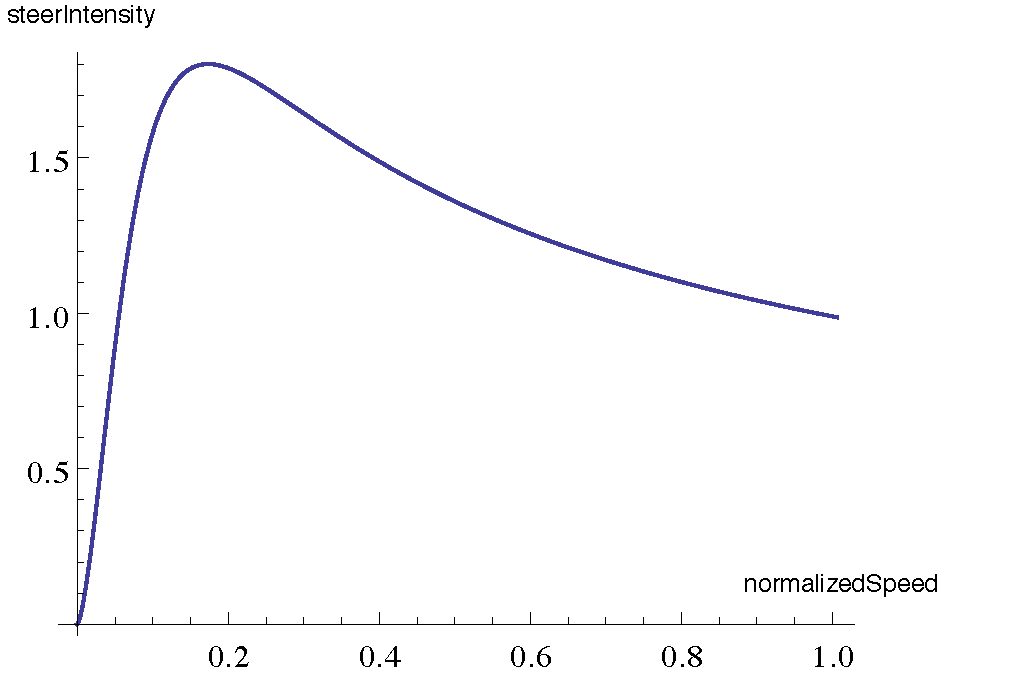
\includegraphics[width=0.7\linewidth]{src/steerIntensity.pdf}
\caption{Steuerintensität in Abhängigkeit der Geschwindigkeit} % Titel der Grafik
\label{steer_intensity} % Labelname
\end{figure}

\subsubsection*{Fahrzeug bewegen}
\begin{lstlisting}[caption={Fahrzeug bewegen},label={fahrzeug_bewegen}]
// update car position
Ogre::Real xMove = Ogre::Math::Sin(carNode->getOrientation().getYaw()) * speed * evt.timeSinceLastFrame;
Ogre::Real zMove = Ogre::Math::Cos(carNode->getOrientation().getYaw()) * speed * evt.timeSinceLastFrame;
carNode->translate(xMove, 0, zMove);
\end{lstlisting}

Die Koordinaten des Autos werden ensprechend seiner Ausrichtung und Geschwindigkeit neu berechnet.

\subsubsection*{Kamera positionieren}
\begin{lstlisting}[caption={Positionierung der 1st-Person-Kamera},label={positionierung_fp_kamera}]
// position camera
Ogre::Vector3 cameraOffset(1.3, 4.0, 0.7);
camera->setOrientation(carNode->getOrientation() * Ogre::Quaternion(Ogre::Degree(180), Ogre::Vector3::UNIT_Y));
camera->setPosition(carNode->getPosition() + carNode->getOrientation() * cameraOffset);
\end{lstlisting}
In der \gls{1st-person}-Ansicht wird die Kamera an die Stelle, an der sich der Kopf des Fahrers befindet verschoben.

\begin{lstlisting}[caption={Positionierung der 3rd-Person-Kamera},label={positionierung_tp_kamera}]
if(gear != REVERSE)
	cameraRotationOffset *= Ogre::Math::Pow(0.1, evt.timeSinceLastFrame);
else
	cameraRotationOffset = cameraRotationOffset * Ogre::Math::Pow(0.1, evt.timeSinceLastFrame) + 180 * (1 - Ogre::Math::Pow(0.1, evt.timeSinceLastFrame));

Ogre::Radian camAngle = carNode->getOrientation().getYaw() + Ogre::Degree(cameraRotationOffset);
Ogre::Real camXOffset = -Ogre::Math::Sin(camAngle) * 25;
Ogre::Real camYOffset = 8;
Ogre::Real camZOffset = -Ogre::Math::Cos(camAngle) * 25;

camera->setPosition(carNode->getPosition() + Ogre::Vector3(camXOffset, camYOffset, camZOffset));
camera->lookAt(carNode->getPosition());

carNode->setVisible(true);
cockpitNode->setVisible(false);
pointerNode->setVisible(false);
steeringWheelNode->setVisible(false);
\end{lstlisting}

Im \gls{3rd-person}-Modus wird die Kamera um eine bestimmte Distanz nach hinten verschoben und zum Mittelpunkt des Fahrzeugs ausgerichtet.




	\section{Resultate und Tests}
\subsection{Erreichtes}
Die Schnittstelle zwischen dem Cockpit und dem Fahrsimulator wurde vollständig in LabVIEW realisiert. Um diese zu testen wurde ein Videoplayer implementiert. Der Videoplayer reagiert auf Eingaben im Cockpit. Beim Drücken des Gaspedals wird das Video schneller, bis maximal doppelt so schnell, abgespielt. Bei einem Druck auf das Bremspedal wird das Video langsamer abgespielt. Liegt die Geschwindigkeit unter 15 km/h, wird das Video pausiert.\\
Im Fahrsimulator kann das Fahrzeug durch Eingaben im Cockpit bewegt werden. Es stehen zwei unterschiedliche Szenen zur Verfügung. Eine Szene stellt eine Stadt dar, in welcher mehrere Strassen, die sich kreuzen, vorhanden sind. Die Kreuzungen sind durch Asphaltsymbole und Verkehrsschilder gekennzeichnet. Um die Stadtszene lebendiger zu machen, sind verschiedene Gebäude und Bäume eingefügt worden. Zudem wurde das ETH Zürich Gebäude in die Szene eingefügt. Dies zeigt exemplarisch, wie einfach Objekte aus dem \gls{google-3d-warehouse} eingefügt werden können. Eine zweite Szene ist ein Rundkurs in einer Berglandschaft. Auf diesem Rundkurs gibt es mehrere Tunnels, die duch die Berglandschaft führen.
Die Daten beider Systeme, die des Videoplayers sowie die des Fahrsimulators, werden erfolgreich an das LabVIEW-Programm zurückgeschikt und in ein Log-File geschrieben. Diese Daten können in eine spätere Auswertung mit einbezogen werden.\\
Somit wurden alle Anforderungen an das Projekt erfüllt. Das Resultat betrachten wir als zufriedenstellend. 
\subsection{Zeitliches Verhalten des Systems}
Es wurden für den Videplayer und den Fahrsimulator Zeitmessungen durchgeführt. Bei beiden Tests war das System auf einer einzigen Maschine installiert. Das Einlesen des Cockpits wurde physisch nicht vom System getrennt. Es gibt also keine Verzögerung durch das Netzwerk. Trotz dieser Tatsache war das Resultat überraschend, denn die Verzögerung liegt im Normalfall unter einer Millisekunde.
\subsection{Testfälle}
Es ist im Allgemeinen schwierig eine grafische Applikation wie ein Fahrsimulator durch automatische Tests zu überprüfen. Deshalb wurden die meisten Tests manuell durchgeführt. Dies geschah jeweils mindestens jeden zweiten Montag Nachmittag während vier bis fünf Stunden. In dieser Zeit wurden alle Neuerungen, die während der Woche entwickelt wurden, auf dem Fahrsimulator installiert und eingehend getestet. \\
Häufige Fehlerursachen waren versäumte Initialisierungen von Variabeln, welche auf verschiedenen Betriebssystemen unterschiedlich gehandhabt werden. Da der Fahrsimulator auf unterschiedlichen Betriebssystemen getestet wurde, konnten diese Fehlerquellen weitgehend eliminiert werden. \\
Wir, das Entwicklerteam, sind durch das häufige Testen zur Überzeugung gekommen, dass die Software den Anforderungen an Stabilität und Zuverlässigkeit gerecht wird.
	\section{Nächste Schritte}
\subsection{Offene Punkte}
Trotz einem gutem Endergebniss der Arbeit, konnten einige Punkte aus Zeitgründen nicht realisiert werden. Einer dieser Punkte ist die implementierung von anderen Verkehrsteilnemern wie zum Beispiel ander Autos, Passanten oder Velofahrer. Zusätzlich hätte dann auch eine Kolisionserkennung implementiert werden müssen, um Zusammenstösse mit ruhenden oder bewegten Objekten zu erkennen. Um der Illusion der realen Welt etwas näher zu kommen, wäre eine implementation eines eigenen \glspl{shader} von grossem Vorteil. Um das Starten des Fahrsimulators zu erleichtern wäre ein \gls{gui} eine gute Lösung gewesen. 
\subsection{Zusätzliche Funktionen}
Um den Fahrsimulator unabhänging von den Szenen zu machen, die manuell erstellt werden müssen, könnten die Szenen aus Informationen von google maps automatisch generiert werden. Auf google maps sind die Informationen über Lage, Art und Richtung der Strasse verfügbar. Ein Algorithmus könnte mit diesen Informationen Strassen für jedes beliebige Gebiet generieren. \\
Eine weitet Zusätzliche Funktion wäre ein erweitertes \gls{gui}, mit dem manipulationen am Fahrzeug vorgenommen werden könnten. Zum Beispiel könnte die Leistung des Fahrzeuges oder die Helligkeit der Szene verändert werden. 
\subsection{Ausblick auf Bachelor Arbeit 2012}
Da die Zusammenarbeit mit der ETH sehr erfolgreich war und das Projekt sehr Zufriedenstellend verlief, wurde von den zuständigen Dozenten die Weiterführung der Projektarbeit als Bachelor Arbeit beschlossen. Wir begrüssen diese Entscheidung sehr und freuen uns dieses Thema noch weiter vertiefen zu dürfen. Wir freuen uns auf eine weiterhin gute und konstruktive Zusammenarbeit. 
	\section{Nachwort}
\subsection{Schlusswort}
Die Projektarbeit Fahrimulator konnte erfolgreich und termingerecht abgeschlossen werden. Sämtliche Anforderungen der Aufgabenstellung wurden erfüllt. Das Fahrzeug kann durch Eingaben im Cockpit navigiert werden und es stehen zwei unterschiedliche Szenen zur Verfügung. Das System läuft weitgehend robust.\\
Mehr Zeit als zu Anfang geplant, benötigten wir vorallem für die Erstellung der verschiedene Szenen. Obwohl wir mit dem Cinema 4D ein sehr gutes Tool zu Hand hatten, mussten Matrialien und Texturen manuell erstellt weden. Dies führte zu Fehlern die wiederum viel Zeit benötigten, um behoben zu werden.\\
Rückblickend sind wir froh, dass wir uns zu Beginn gegen einen Einsatz von google maps und google Street View entschiden haben. Durch die eingene modelierung der 3D Umgebungen konnten so gute Resultate erziehlt werden, wie sie mit den beiden anderen Tools niemals möglich gewesen wären. 
\subsection{Danksagung}
An dieser Stelle möchten wir unseren beiden Projektbetreuern  Prof. Dr. Peter Früh und Prof. Martin Schlup danken für ihre Betreuung, Unterstüzung und Anregungen während der gesamten Projektarbeit. Ebenso möchten wir dem Team an der ETH Zürich, Ying-Yin Huang und Prof. Dr. Marino Menozzi für eine erfolgreiche und angenehme Zusammenarbeit danken. Des weiteren danken wir Daniela Zehnder und Katrin Achtnich für die Überprüfung der Rechtschreibung und Grammatik. 

	
	% anhang
	%\renewcommand{\thesection}{\Alph{section}}
	%\setcounter{section}{0}
	\appendix
	
	\fancyhead[RE]{Anhang \leftmark}
	\section{Aufgabenstellung}
\begin{figure}[h]
	\flushleft
	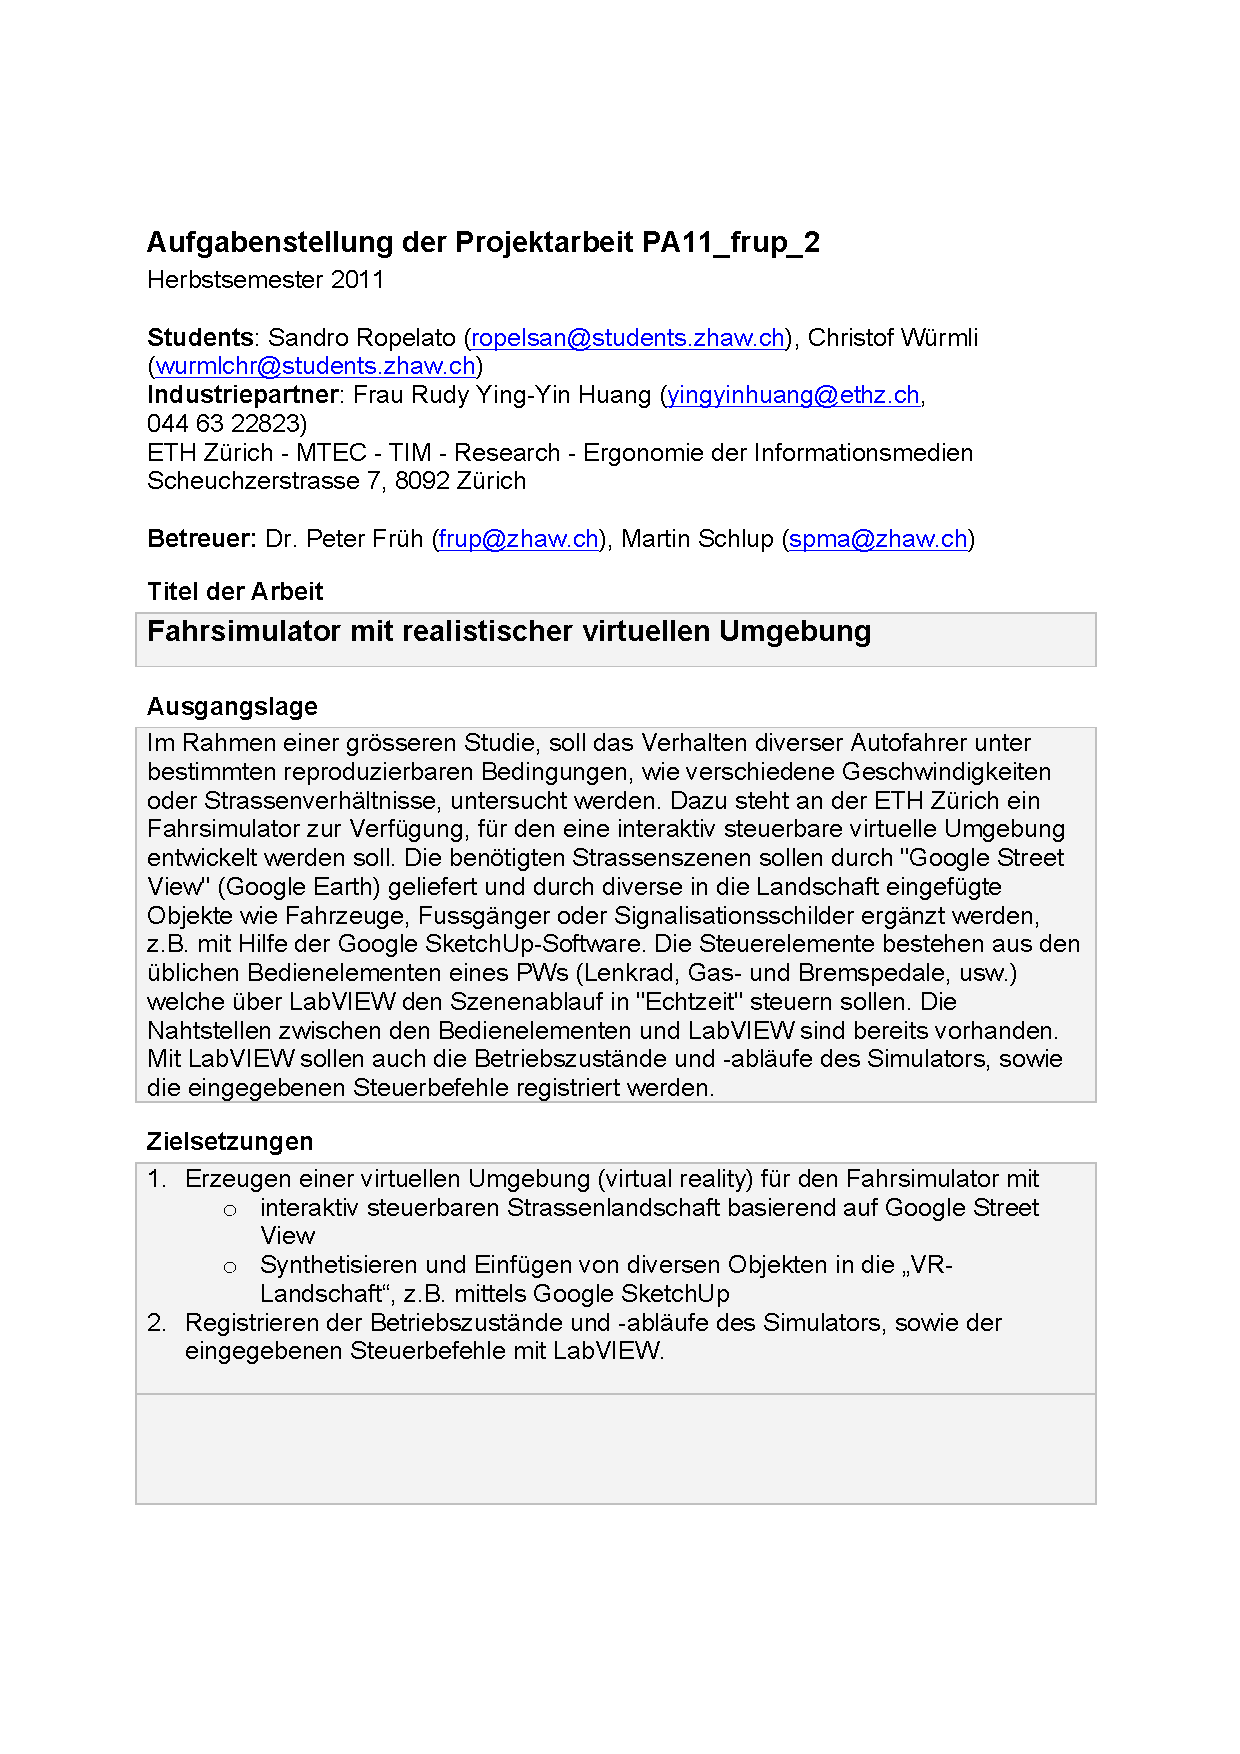
\includegraphics[width=\linewidth]{src/aufgabenstellung_seite1.pdf}
\end{figure}
\begin{figure}[h]
	\flushleft
	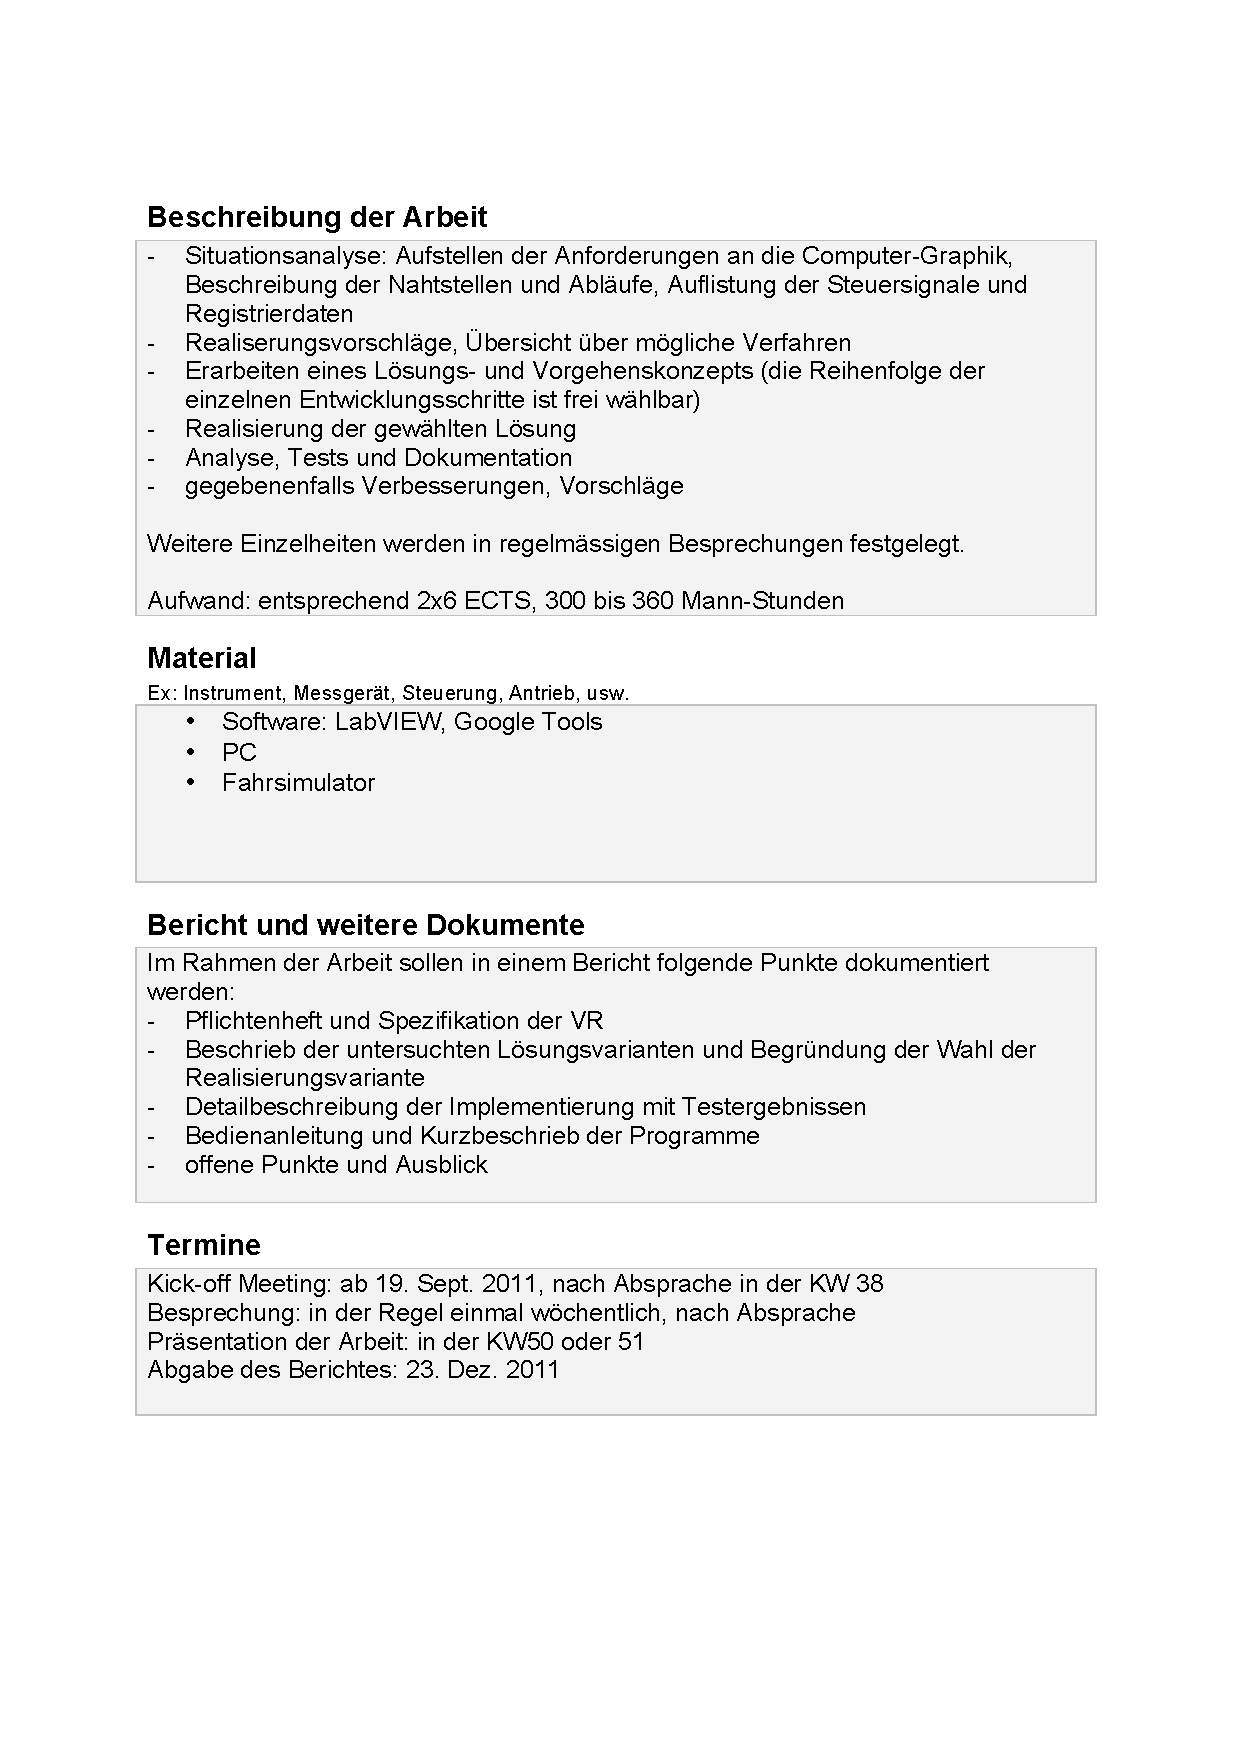
\includegraphics[width=\linewidth]{src/aufgabenstellung_seite2.pdf}
\end{figure}


	\section{Videoplayer}
\subsection{Ziel}
In einem ersten Schritt, vor der Realisierung des Fahrsimulator, wird ein Videoplayer ralisiert. Das Ziel dabei ist der Aufbau und Test der Anbindung der Eingabehardware an unser Programm. Bei der Betätigung des Gaspedals im Cockpit soll das aufgenommene Video schneller abgespielt werden. Bei der Betätigung des Bremspedals dementsprechend langsamer. Der Videoplayer soll so aufgebaut werden, dass Komponenten davon auch im Fahrsimulator wiederverwendet werden können. Die ETH Zürich besitzt bereits Videos, die sich gut dafür eigenen. Um Experimente mit diesen Videos durchführen zu können, müssen Eingaben, die der Proband im Cockpit mach, mit der aktuellen Position des Videos abgespeichert werden. Dies dient zur späteren Auswertung der Experimente.
\\
\subsection{Systembeschreibung}

Um einzelne Komponenten des Videoplayer wiederverwenden zu können, wird das System möglichst gleich wie das des Fahrsimulators aufgebaut. Dieser Aufbau wird anhand der Abbildung \ref{Systembeschreibung Videoplayer} illustriert. Blau markiert sind neu entwickelte Komponenten des Videoplayers. Die Eingaben im Cockpit werden von einem LabVIEW-Programm über eine USB-Schnittstelle eingelesen. Die eingelesenen Parameter werden, zusammen mit einem Timestamp, von LabVIEW in ein UDP-Paket verpackt und über einen UDP-Socket gesendet. Das Paket wird von einem UDP-Listener empfangen und gelesen. Dieser speichert die Daten ab und hält sie für das Hauptprogramm bereit. Das Hauptprogramm (Main Application) liest die gespeicherten Parameter aus und interpretiert diese. Der \gls{mplayer}, der für das Abspielen der Videos verwendet wird, lässt sich durch Konsoleneingaben über die Standard-In-Pipe steuern. So wird ihm vom Videoplayer mitgeteilt, wie schnell das aktuelle Video abgespielt werden soll.  Über die Standard-Out-Pipe gibt MPlayer die aktuelle Abspielposition zurück. Das Hauptprogramm wertet diese aus, ergänzt sie mit Benutzereingaben und leitet sie über den UDP-Listener an LabVIEW weiter. Dort werden die Daten über  einen zweiten UDP-Socket empfangen und für eine spätere Auswertung in ein Log-File gespeichert.
\newpage

% Bild für Systembeschreibung des Video Players
\begin{figure}[H]
\centering 
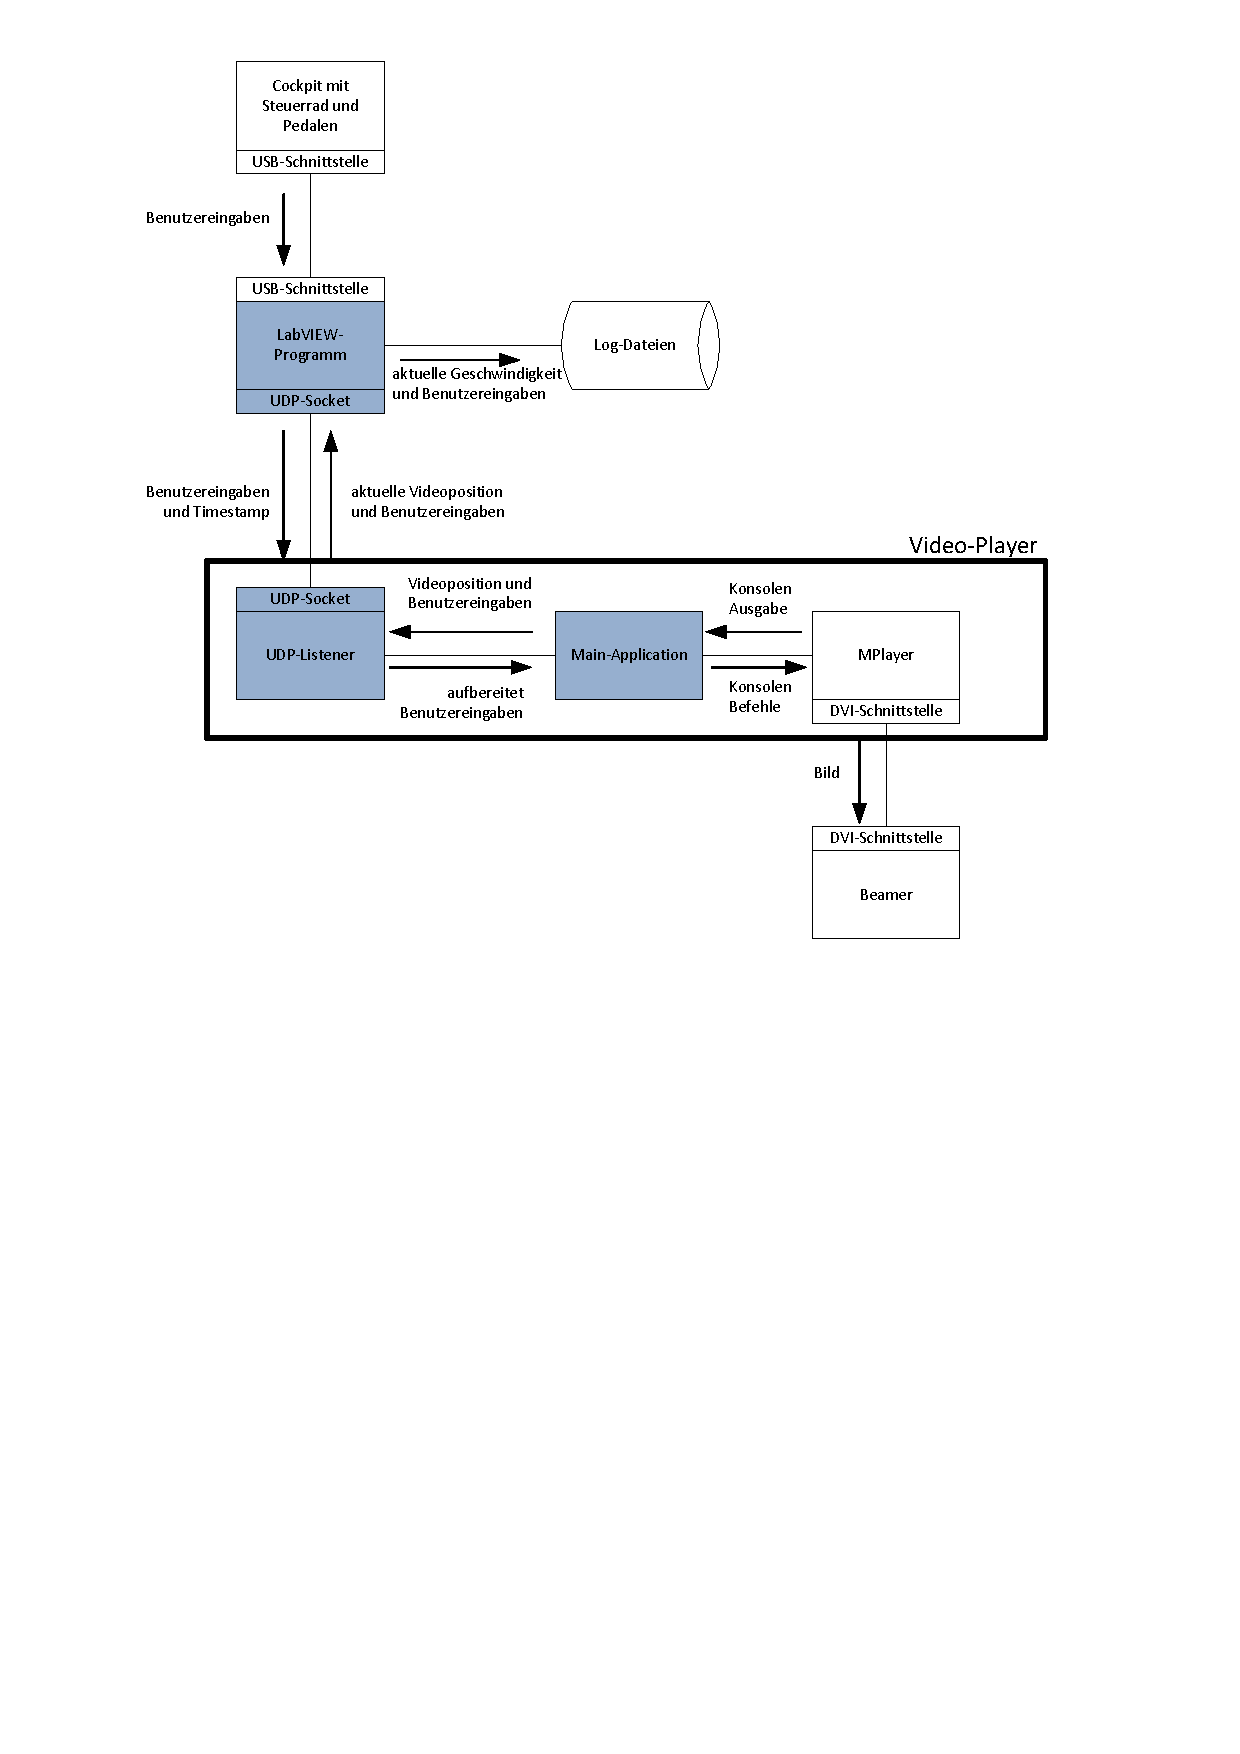
\includegraphics[width=0.8\linewidth]{src/Systembeschreibung_VideoPlayer.pdf}
\caption{Systembeschreibung Videoplayer} % Titel der Grafik
\label{Systembeschreibung Videoplayer} % Labelname
\end{figure}

\subsection{Realisierung}
Bei der Realisierung des Videoplayers wird der Fokus vorallem auf die Entwicklung der LabVIEW-Schnittstelle zu unserem Programm gelegt. Darum wird dieser Schritt nachfolgend ausführlich erklährt. Diese Schnittstelle wird auch für den Fahrsimulator selbst verwendet.

\subsubsection{LabVIEW-Schnittstelle}
\label{labview_schnittstelle}
Die Realisierung der LabVIEW Schnittstelle wird in zwei Teile unterteilt. Der erste Teil dient dazu, die Benutzereingaben einzulesen und an den UDP-Listener zu senden. Der zweite Teil befasst sich mit dem Empfangen von Daten, die vom UDP-Listener gesendet werden und deren Speicherung in ein Log-File.

\newpage 

% LabVIEW Screenshot, Daten senden
\begin{figure}[H]
\centering 
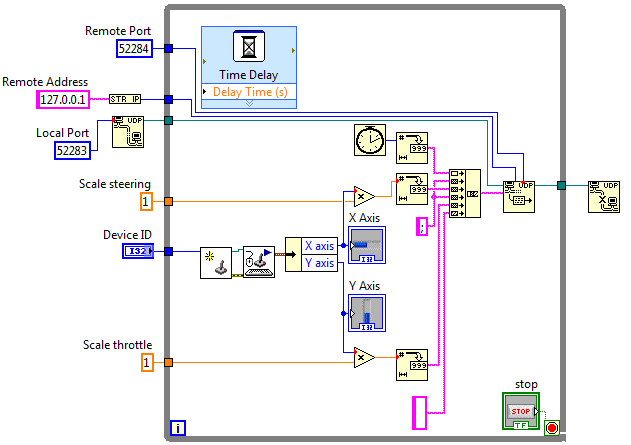
\includegraphics[width=1\linewidth]{src/labview_screenshot_videoplayer_daten_senden.png}
\caption{Einlesen und Versenden der Daten mit LabVIEW} % Titel der Grafik
\label{labview_screenshot_videoplayer_daten_senden} % Labelname
\end{figure}
Die Abbildung \ref{labview_screenshot_videoplayer_daten_senden} illustriert den Aufbau des LabVIEW-Programms, mit dem Eingaben vom Cockpit eingelesen und über einen UDP-Socket versendet werden. Das Verhalten des Programms kann über diverse Parameter geändert werden.\\
Die \textit{Remot Address} gibt an, an wen die UDP-Pakete gesendet werden. Da sich der UPD-Listener zur Zeit auf dem selben Rechner wie dieses Programm befindet, wählen wir hierfür die Localhost-Adresse 127.0.0.1. Für den \textit{Remote Port} wählen wir einen freien Port, hier 52284. Zusammen mit dem \textit{Local Port}, der uns eine Verbindungs-ID generiert, ist unsere Konfiguration für den UDP-Socket vollständig. Um die Komponenten im Cockpit ansprechen zu können, muss lediglich die richtige \textit{Device ID} gewählt werden. Die anderen Komponenten, die sich in der grauen Box befinden, werden in einer Schleife 100 mal pro Sekunde ausgeführt. Dieser Wert wird mit dem Element \textit{Time Delay} konfiguriert.\\
Aus dem Cockpit werden die Werte der x- und y-Achse des Joysticks eingelesen. Auf der y-Achse werden die Werte der beiden Pedalen abgebildet. Ein negativer Wert quantiviziert hierbei das Drücken des Gaspedals, ein positiver Wert das Drücken des Bremspedals. Die Intensität beider Pedalen wird im Positiven durch 32767 und im Negativen durch 32768 ganzzahlige Werte abgestuft. Ein voll gedrücktes Gaspedal entspricht also dem Wert -32768 auf der y-Achse und ein voll gedrücktes Bremspedal entspricht dem Wert 32767. Die x-Achse quantifiziert analog dazu den Einschlagswinkel des Steuerrades. Hierbei ist, wenn das Steuerrad sich in der neutralen Position befindet, der x-Wert null. Komplett nach rechts eingeschlagen beträgt der x-Wert 32767 und -32768 bei einem Einschlag nach links. Der x-Wert wird ebenfalls ausgelesen, ist aber im Video-Player nicht relevant. Die beiden Werte werden je mit einem separaten Faktor multipliziert, um eventuell eine Anpassung derjenigen vorzunehmen. Danach werden sie zusammen mit dem aktuellen Timestamp durch Semikolons voneinander getrennt, in das UDP-Paket gepackt und dann versendet. Nach Verlassen der Schleife wird der UDP-Socket wieder geschlossen.

Die Abbildung \ref{labview_screenshot_videoplayer_daten_empfangen} illustriert den Aufbau des LabVIEW-Programms, mit dem die Daten vom Videoplayer empfangen und in ein Log-File gespeichert werden.\\
Es wird ein UDP-Socket geöffnet um ankommende Pakete zu empfangen. Der \textit{Local port} mit dem UDP-Verbindungskästchen generiert wieder eine Connection-ID, die für das Öffnen des UPD-Ports benötigt wird. Durch die Angaben von \textit{Maximum datagram size} und \textit{Timeout} wird der UPD-Socket so konfiguriert, dass er nur Packete kleiner als 4096 Bytes liest und höchstens 500 ms auf das Eintreffen eines Pakets wartet. Ist die Übertragung des Pakets fehlerhaft ist oder dauert sie zu lange, wird abgebrochen und auf das nächste Paket gewartet. Der hierbei von LabVIEW erzeugte Fehler wird ignoriert.\\
Bei einer erfolgreichen Übertragung liegen die Daten als eine Zeichenkette vor. Die einzelnen Werte in der Zeichenkette sind mit Semikolons voneinander getrennt. Diese Zeichenkette wird jetzt weiterverarbeitet. Die beiden Filmstreifenfenster bewirken, dass die Aktionen im zweiten Fenster erst ausgeführt werden, wenn die im ersten Fenster erzeugten Daten vollständig vorliegen. Dies ist vorallem für den Timestamp, der wieder von der Uhr kommt, wichtig, da dieser erst erstellt werden darf, wenn das Packet gelesen wurde. Die Werte werden voneinander getrennt und die Semikolons gelöscht. Sie repräsentieren nun verschiedenste Eigenschaften des Systems. So ist zum Beispiel der dritte Wert die aktuelle Geschwindigkeit des Fahrzeuges. Dieser Wert wird benötigt um auf der Benutzeroberfläche die Geschwindgkeit in einem Tacho anzuzeigen. Zudem wird auch der vierte Wert benötigt um die aktuelle Abspielposition des Videos auszugeben. Alle Werte, inklusive der aktuellen Position von Pedalen und Steuerrad, werden nun, wieder getrennt durch Semikolons, zu einer Zeichenkette zusammengefügt. Diese wird dann laufend in einem File gespeichert. Die erste Zeile des Files ist ein Header und beschreibt die Felder. Er wird in der Abbildung \ref{labview_screenshot_videoplayer_daten_empfangen} unten links zusammengestellt. Nachdem die Schleife beendet wurde, werden UDP-Socket und File geschlossen.

\newpage

% LabVIEW Screenshot, Daten empfangen
\begin{figure}[H]
\centering 
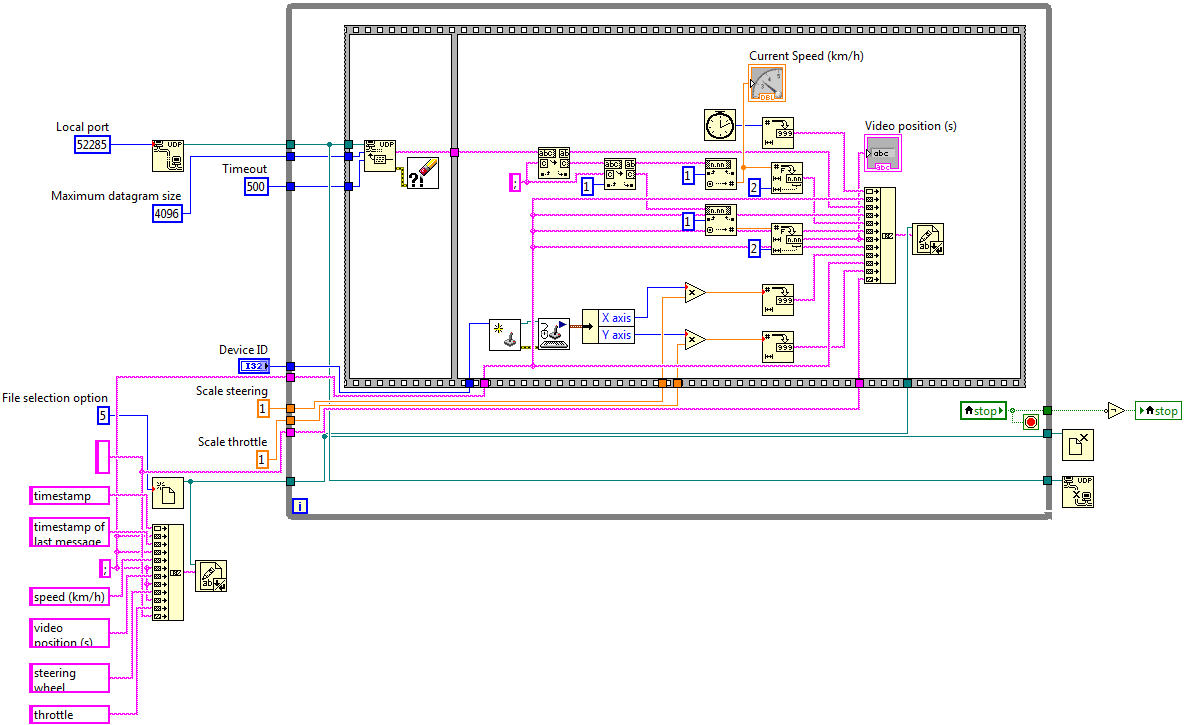
\includegraphics[angle=90,width=0.9\linewidth]{src/labview_screenshot_videoplayer_daten_empfangen.png}
\caption{LabVIEW: Daten empfangen} % Titel der Grafik
\label{labview_screenshot_videoplayer_daten_empfangen} % Labelname
\end{figure}

\newpage

\subsubsection{UDP-Listener}
Der UDP-Listener empfängt die Pakete, die von LabVIEW gesendet werden. Diese werden ausgepackt und die übermittelten Werte abgespeichert. Der UDP-Listener wird im Kapitel \ref{sec:udp-listener} genau dokumentiert.
\subsubsection{Hauptprogramm}
Das Hauptprogramm startet den MPlayer und den UDP-Listener. Der MPlayer wird, um ein Video abzuspielen, in einem eigenen Prozess gestartet und kann duch Aufrufe über die Standard-In-Pipe, wie im Listing \ref{start_mplayer} beschrieben, im Slavemodus gestartet werden. Wie der MPlayer im Videoplayer aufgerufen wird, kann dem Quellcode auf der beiliegenden DVD entnommen werden. 
\begin{lstlisting}[caption={Starten des MPlayers in einem eigenen Prozess}, label={start_mplayer}]
mplayer.exe -slave -hardframedrop -osdlevel 0 BeispielVideo.mp4
\end{lstlisting}
Der Parameter \textit{hardframedrop} dient der Erhöhung der Framerate. Es erlaubt dem Player bei hohen Abspielgeschwindigkeiten einzelne Bilder auszulassen um so eine höhere Framerate zu erzielen. Der \textit{osdlevel} Parameter bestimmt wieviel Information auf dem Bildschrim angezeigt wird. Der Level null unterdrückt alle Ausgaben.\\
In diesem Slavemodus nimmt der MPlayer Befehle die über die Standard-In-Pipe entgegen und schreibt seine Ausgabe in die Standard-Out-Pipe. Dazu werden die beiden Pipes des MPlayer-Prozesses im Hauptprogramm verfügbar gemacht und erlauben so eine Kommunikation der beiden Programme. 
\begin{lstlisting}[caption={Funktion zum Senden von Nachrichten an MPlayer}, label={mplayer_befehl}]
int sendMessage(const char* message)
{
	DWORD dwWritten;
	if(!WriteFile(stdInWr, message, strlen(message), &dwWritten, NULL))
	{
		fprintf(stderr, "Could not write to pipe.\n");
		return 1;
	}
	return 0;
}
\end{lstlisting}
Im Listing \ref{mplayer_befehl} quantifiziert \textit{speed} die Abspielgeschwindigkeit in der das Video abgespielt werden soll. 
	\section{Das OGRE-Framework}

\subsection{Was ist das OGRE-Framework}

\begin{wrapfigure}{r}{0.4\linewidth}
	
\includegraphics[width=1\linewidth]{src/OgreLogo.png}
	\caption{OGRE Logo} % Titel der Grafik
	\label{OGRE Logo} % Labelname
\end{wrapfigure}

OGRE (Object-Oriented Graphics Rendering Engine) ist eine Grafikengine zur Echtzeitdarstellung von dreidimensionalen Szenen. Sie ist in C++ geschrieben und ihre Verwendung unterliegt der MIT-Lizenz. Durch den modularen Aufbau und die Unterstützung auf verschiedenen Plattformen erweist sich OGRE als sehr flexibel und mächtig. OGRE selbst benutzt die Grafikbibliotheken \gls{opengl} und \gls{directx} zum hardwarebeschleunigten Rendern der Szenen und setzt automatisierte Optimierungsalgorithmen zur Geschwindigkeitsgewinnung ein. Mittlerweile existiert eine grosse und aktive Community, welche das OGRE-Framework ständig weiter entwickelt und verbessert.

\subsection{Weshalb setzen wir OGRE ein?}

Im Vergleich zur direkten Verwendung von \gls{opengl} oder \gls{directx} bringt der Einsatz einer Grafikengine wie OGRE eine Vielzahl von Vorteilen mit sich:

\minisec{Abstraktion} \gls{opengl} und \gls{directx} sind zwei komplett verschiedene Bibliotheken. Hat man sich für eine von beiden entschieden, so bedeutet das Umsteigen auf eine andere unter Umständen das Neuschreiben des kompletten Codes. OGRE abstrahiert die Verwendung dieser Grafikbibliotheken und ermöglicht den selben Code entweder mit OpenGL oder DirectX laufen zu lassen.

\minisec{Geschwindigkeit} text


	\section{Betriebsanleitung}
Hier wird in einer kurzen Schritt-für-Schritt-Anleitung erklärt, wie die Applikationen \textit{VideoPlayer} und \textit{DrivingSimulator} zu bedienen sind.
\subsection{VideoPlayer}
Der VideoPlayer benötigt eine funktionierende Installation des Programms MPlayer. MPlayer kann auf der Herstellerseite (http://www.mplayerhq.hu) kostenlos heruntergeladen werden.

\begin{enumerate}[label=\arabic*.]

\item \textbf{LabVIEW-Programm starten}\\
Öffnen Sie die Datei VideoPlayer.vi mit LabVIEW und starten Sie das Programm mit einem Klick auf die Schaltfläche 
\includegraphics[height=\ht\strutbox]{src/icon_labview_run.png} \textit{Run}. Sie werden nach einem Dateipfad gefragt. Geben Sie hier den Pfad zu einer Datei an, in der Sie den Output vom LabVIEW-Programm gespeichert haben wollen. \textbf{Achtung: Existierende Dateien werden überschrieben!}

\item \textbf{VideoPlayer starten}\\
Starten Sie \textit{VideoPlayer2.exe} entweder direkt von der Kommandozeile mit folgenden Parametern in der Reihenfolge, wie sie hier aufgelistet sind:
\begin{itemize}
	\item Pfad zu mplayer.exe
	\item Pfad zur Videodatei
	\item Startzeit der gewünschten Videosequenz (in Sekunden)
	\item Endzeit der gewünschten Videosequenz (in Sekunden)
	\item Referenzgeschwindigkeit, d.h. Geschwindigkeit mit der das Video aufgenommen wurde (in km/h)
	\item UDP Input Port
	\item UDP Output Port
	\item Adresse des Remote Computers ("127.0.0.1" wenn das LabVIEW-Programm auf demselben Computer läuft)
\end{itemize}
oder benutzen Sie die Datei \textit{VideoPlayer2.bat}, welche bereits mit den Standardwerten konfiguriert ist und ein beigelegtes Beispielvideo abspielt.
	
\item \textbf{Los gehts}\\
Setzen Sie sich nun ans Steuer und kontrollieren Sie die Geschwindigkeit des Fahrzeugs durch drücken des Gas- bzw. Bremspedals. Die aktuelle Geschwindigkeit und Position im Video wird im LabVIEW-Programm angezeigt. Alle Informationen werden, solange das Programm läuft, in die, in Schritt 1 angegebene, Datei geschrieben.

\end{enumerate}

\newpage
\subsection{Fahrsimulator}
Der Fahrsimulator benötigt DirectX 9 um zu laufen. Falls Sie dies noch nicht installiert haben, können Sie es von der offiziellen Microsoft-Seite\footnote{http://www.microsoft.com/download/en/details.aspx?id=8109} herunterladen: 

\begin{enumerate}[label=\arabic*.]

\item \textbf{LabVIEW-Programm starten}\\
Öffnen Sie die Datei DrivingSimulator.vi mit LabVIEW und starten Sie das Programm mit einem Klick auf die Schaltfläche 
\includegraphics[height=\ht\strutbox]{src/icon_labview_run.png} \textit{Run}. Sie werden nach einem Dateipfad gefragt. Geben Sie hier den Pfad zu einer Datei an, in der Sie den Output vom LabVIEW-Programm gespeichert haben wollen. \textbf{Achtung: Existierende Dateien werden überschrieben!}

\item \textbf{Grafikeinstellungen überprüfen}\\
Öffnen Sie die Datei \textit{Resources/graphics.cfg}. Darin befinden sich einige Attribute für die Grafikkonfiguration. Vergewissern Sie sich, dass Ihre Grafikkarte die dort spezifizierten Grafikmodi unterstützt und ändern Sie diese gegebenenfalls ab. Die wichtigsten Optionen sind hier aufgeführt:
\begin{itemize}
	\item Video Mode: Bildschirmauflösung und Farbtiefe in folgendem Format: \textit{<horizontale Auflösung> x <vertikale Auflösung> @ <Farbtiefe>-bit colour}\\Beispiel: \textit{1024 x 768 @ 32-bit colour}
	\item FSAA: Anzahl Filterdurchgänge für Antialiasing (\textit{0}, \textit{2}, \textit{4}, \textit{8}, etc.)
	\item Full Screen: \textit{Yes} oder \textit{No}
	\item VSync: Bildschirmsynchronisation aktivieren (\textit{Yes} oder \textit{No})
\end{itemize}

\item \textbf{Fahrsimulator starten}\\
Wechseln Sie zuerst in das Verzeichnis, in dem sich die Date \textit{DrivingSimulatorV1.exe} befindet und starten Sie diese entweder direkt von der Kommandozeile mit folgenden Parametern in der Reihenfolge, wie sie hier aufgelistet sind:
\begin{itemize}
	\item UDP Input Port
	\item UDP Output Port
	\item Adresse des Remote Computers ("127.0.0.1" wenn das LabVIEW-Programm auf demselben Computer läuft)
	\item Rückwärtsgang (\textit{1}: aktiviert, \textit{0}: deaktiviert) 
	\item Steuerrad (\textit{1}: sichtbar, \textit{0}: unsichtbar)
	\item Level (\textit{1}: Stadtszene, \textit{2}: Berglandschaft)
\end{itemize}
oder benutzen Sie die Dateien \textit{DrivingSimulator\_City.bat} oder\\
\textit{DrivingSimulator\_Mountains.bat}, um eine entsprechende Szene mit Standardeinstellungen zu laden.

\item \textbf{Los gehts}\\
Setzen Sie sich nun ans Steuer und fahren Sie durch die virtuelle Welt. Das Fahrzeug kann über Eingaben im Cockpit oder durch die Pfeiltasten gesteuert werden. Durch Drücken der Taste \textit{V} auf der Tastatur, wird die Kameraansicht zwischen 1st- und 3rd-Person umgestellt.


\end{enumerate}

	\section{Screenshots}

	\section{Detaillierter Zeitplan}
\label{detaillierter_zeitplan}

\begin{figure}[H]
\centering 
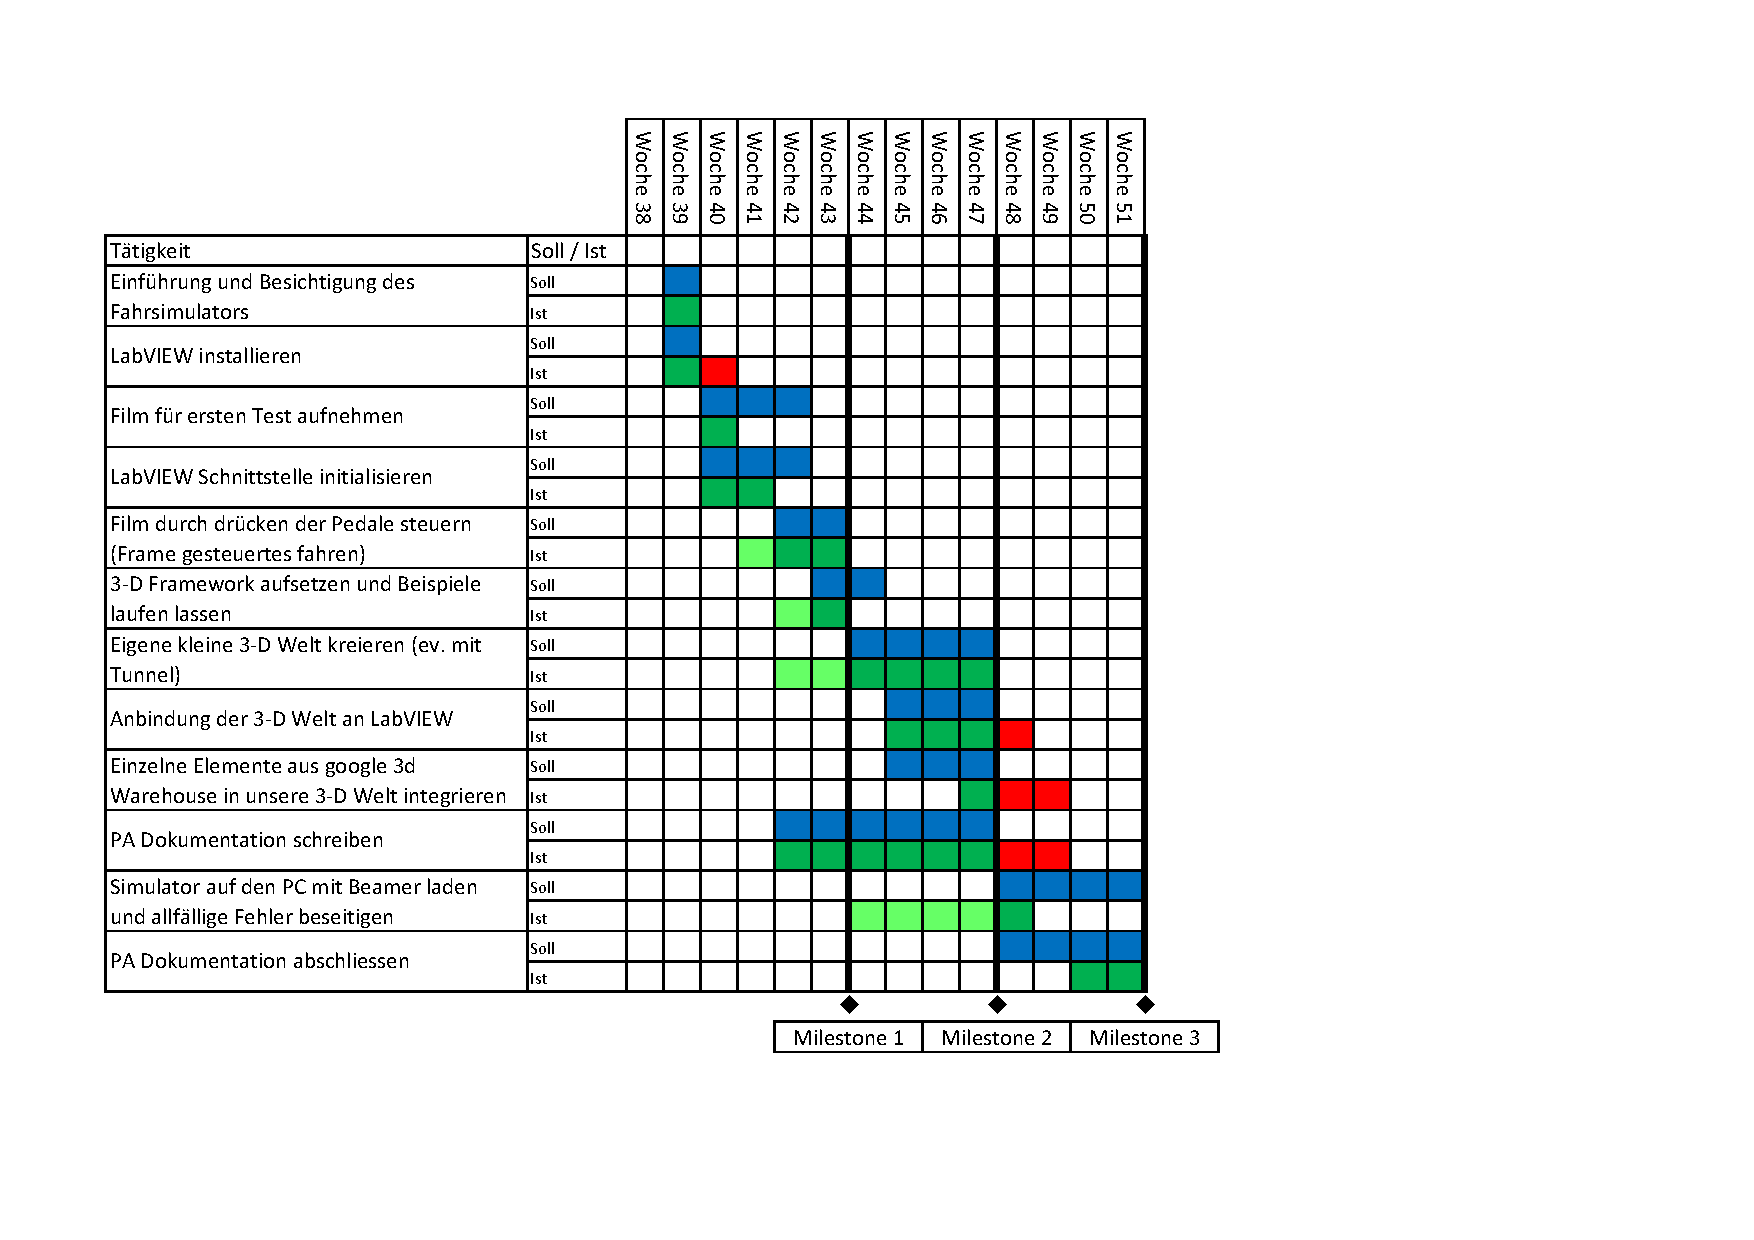
\includegraphics[width=1.0\linewidth]{src/Zeitplan.pdf}
\caption{Detailierter Zeitplan} % Titel der Grafik
\label{zeitplan} % Labelname
\end{figure}
\minisec{Einführung und Besichtigung des Fahrsimulators}
Der Aufbau des Fahrimulators und die Softwareumgebung wird besichtigt. Da das Projekt für die ETH durchgeführt wird, werden die Verantowrtlichen vorgestellt und mit ihnen Ziele und Anforderungen an die Arbeit besprochen. 
\minisec{LabVIEW installieren}
Das LabVIEW Programm wird auf unseren privaten Rechnern installiert. Wir machen uns damit vertraut können es für die Arbeit verwenden. 
\minisec{Film für ersten Test aufnehmen}
Um einen ersten Test mit einem Video-Player machen zu können wird ein geeignetes Video benötigt. Das Video zeigt Aufnahmen von einer Autofahrt und beinhaltet vorzugsweise eine Tunneleinfahrt.

\newpage

\minisec{LabVIEW-Schnittstelle initialisieren}
Im LabVIEW wird eine Schnittstelle eingerichtet um, die Werte des Cockpits in den Fahrsimulator zu übertragen. Entsprechend wird ein Gegenstück entwickelt um die Werte, die von LabVIEW gesendet werden, zu empfangen. 
\minisec{Film durch drücken der Pedale steuern (framegesteuertes fahren)}
Realisation eines Video Players, der einen Film abspielt. Die Abspielgeschwindigkeit wird durch das Drücken des Gas- oder Bremspedals im Cockpit beeinflusst. Beim drücken des Gaspedals wird der Film schneller und beim Bremspedal langsamer. 
\minisec{3D-Framework aufsetzen und Beispiele laufen lassen}
Für die Entwicklung des Fahrsimulators wird ein 3D-Framework mit dem Namen OGRE verwendet. Dies soll in diesem Arbeitsschritt aufgesetzt, konfiguriert und getestet werden. Nach erfolgreichem Testen wird eine kurze einfache Szenen, die nur eine gerade Strasse enthält, erstellt. Die Szene wird aus dem Blickwinkel des Fahrers oder aus der Vogelperspektive gesehen. Zu Testzwecken soll das Fahrzeug mit den Pfeiltasten der Tastatur gesteuert werden.
\minisec{Eigene kleine 3D-Welt kreieren (ev. mit Tunnel)}
Es wird eine eigene 3D-Welt kreiert. Diese Szene kann bereits ein Tunnel enthalten. 
\minisec{Anbindung der 3D-Welt an LabVIEW}
In diesem Arbeitsschritt werden die LabVIEW Schnittstelle und die 3D-Welt zusammengefügt. Danach ist es möglich, das Fahrzeug in der Simulation durch Manipulation im Cockpit zu steuern. 
\minisec{Einzelne Elemente aus Google 3D Warehouse in unsere 3D-Welt integrieren}
Es werden Objekte aus dem Google 3D Warehous in die 3D-Welt integriert, um die Umgebung noch realistischer zu gestalten. 
\minisec{Dokumentation schreiben}
Mit der Dokumentation wird in der zweiten Hälfte der zur Verfügung stehenden Zeit begonnen. Die Besprechungen mit dem ETH Team oder den internen Betreuern werden von Beginn an protokolliert.
\minisec{Simulator auf den PC mit Projektor laden und allfällige Fehler beseitigen}
Der getestete Fahrsimulator wird definitiv auf den Rechner geladen und getestet. Kleinere Fehler und Unschönheiten werden noch beseitigt. 
\minisec{Dokumentation abschliessen}
Die Dokumentation wird von mehreren Personen gegengelesen, korrigiert und die definitive Version dann ausgedruckt und abgegeben. 
	\section{Listings}

\subsection{Drivingsimulator}
\subsubsection{Konfigurationfiles}

\label{listing:plugins.cfg}
\lstinputlisting{listings/plugins.cfg}

\label{listing:graphics.cfg}
\lstinputlisting{listings/graphics.cfg}

\label{listing:resources.cfg}
\lstinputlisting{listings/resources.cfg}

\subsubsection{.h und .cpp Files}

\label{listing:DrivingSimulatorV1.h}
\lstinputlisting{listings/DrivingSimulatorV1.h}
\label{listing:DrivingSimulatorV1.cpp}
\lstinputlisting{listings/DrivingSimulatorV1.cpp}

\label{listing:DrivingSimulatorV1.h}
\lstinputlisting{listings/DrivingSimulatorV1.h}
\label{listing:DrivingSimulatorV1.cpp}
\lstinputlisting{listings/DrivingSimulatorV1.cpp}


	\section{Journal}
\subsection*{26.09.2011}
The driving simulator with steering wheel and pedals is connected to the computer. There is a LabVIEW interface which reads the input from the devices. In a first step, Rudy would like to have a driving controlled only by the pedals. --> modified frame rate \\
After this she'd like to have a driving simulator with focus on tunnel entrances an exits.  
\subsection*{03.10.2011}
The driving simulator may be a fantasy environment or it could be a copy of a real environment. \\
Google Street View is no possibility to generate a 3D world because there are too many distraction in it. For example the other cars, people and traffic jam. The street view does not clearly distinguish between street and surfaces of other objects. Also sometimes there are only pictures available on the wrong side of the street. Another argument not to use Google Street View is that there are too larg distances between the single pictures, so the rendering is not fluent.\\
We would like to use the information from Google Earth to build a city like Zurich. We could use the street location information to build our own streets and then try to render already existing 3D models from Google 3D Warehouse into our virtual world. \\
There is a difficulty about Google Earth when it comes to creating scenes that take place in a tunnel since there is no height information available. A Possibility could be to implement it manually or to ignore spots which cause such problems. If we implement it manually we should define a fixed area where no problems occur. \\
We decided to use UDP sockets to extract data out of LabVIEW into our program and an external video player application to control the video.\\
In a first step we use LabVIEW to control an external application which plays a video with a configurable framerate. 
\subsection*{10.10.2011}
The journal and the timetabele have been set up and seem to be okay. There has to be an English version of the timetable so Rudy can follow the progress made in the project. \\
We have agreed on creating our own 3D world and extend it with some buildings from Google 3D Warehouse. There are already tons of finished 3D models of different buildings. We have to build the streets by ourselves because the streets in Google Earth are not as good as we need them. We will also create a tunnel in our own 3D world, which is impossible when rendering a scene with material of Google Street View. \\
We have presented the video we controlled with LabVIEW and the OGRE framework we would like to use. 
\subsection*{17.10.2011}
We have to calculate the delay time of the user interaction. A timestamp would be very helpful to study the delays. That's important for Rudy's further studies. \\
The video is now controlled by the pedals, and played in MPlayer. There is a batch file to start the application with different videos.
We switched our repository to github because there it's easier to maintain.  
\subsection*{07.11.2011}
It should be possible to get this work further as our Bachelor thesis.\\
We have brought up some ideas to build streets and cities dynamically with little pieces of street tales. \\
We also could create a city (or at least a map) by ourselves. It is only useful to use Google Street View or Google Maps if it bring a remarkable time advantage over doing the scenes manually.\\
Rudy told us some scenarios which she'd like to have for her studies. We will try to create the most of them but we have decided that if there are some elements in it which are animated or have to be controlled from outside, for example another car, we will move it to the Bachelor thesis.  \\
We agreed on building a tunnel scene but won't be able to create a controllable second car moving through that scene. 
\subsection*{14.11.2011}
Today we agree on a set of features that have to be included in the software we will deliver as the result of our project. Namely, these are:
\begin{itemize}
\item Logging of the timestamp in the VidePlayer application
\item Integration of a cockpit view with speedometer
\item Small city map
\end{itemize}
After having completed these tasks we will focus on updating the documentation and making a deliverable version of the software.\\
Tasks to be included in the Bachelor thesis will be discussed in the meeting of the 28th November.
\subsection*{21.11.2011}
We have got different ideas, we would like to implement in the Bachelor thesis. Important about these ideas is a relevance for the experiment they do with the driving simulator. \\
Rudy also gave us a lot of points we could implement in a further work. These are things like a bigger scene simulating an area in Zurich around the airport including the Bubenholz tunnel.  
\subsection*{05.12.2011}
A simple goal of the Bachelor thesis has been set up and we named different possible tasks for it. \\
We discussed the structure we had set up for the PA documentation and got some good hints from Mr. Früeh and Mr. Schlup. There has been a short interview with Prof. Menozzi on a Swiss television programme about his studies. Our driving simulator has been mentionned and shown on TV\footnote{http://www.videoportal.sf.tv/video?id=9410c439-0c70-4ee2-895c-f9339ec2809d}.
\subsection*{12.12.2011}
We verified the definitive structure of the PA documentation. We settled the closing date for the documentation on the 23.12.2011. We are on the right way and absolutely on time with our work.

	
	% verzeichnisse
	\fancyhead[RE]{\leftmark}
	\section{Glossar}

\minisec{LabVIEW} Erklärung
\minisec{Log-Datei} Erklärung
\minisec{Cockpit} Erklärung
	\newpage
	\renewcommand{\cftfigpresnum}{Abbildung }
\renewcommand{\cftfigaftersnum}{:}
\setlength{\cftfigindent}{0mm}
\setlength{\cftfignumwidth}{25mm}

\addcontentsline{toc}{section}{\listfigurename}
\listoffigures

	
\end{document}
